\documentclass[preprint]{elsarticle}
\usepackage{amssymb}
\setcounter{tocdepth}{3}
\usepackage{graphicx,epsfig}
\usepackage{graphicx}
\usepackage{algorithm}
\usepackage{algorithmic}
%\usepackage{listings}
\usepackage{rotating}
\usepackage{subfigure}
\usepackage{multirow}
\usepackage{fancyvrb}
%\usepackage[boxed]{algorithm2e}l
%\usepackage{algpseudocode}

\providecommand{\SetAlgoLined}{\SetLine}
\providecommand{\DontPrintSemicolon}{\dontprintsemicolon}
%%%%

\usepackage{color}
\usepackage{alltt}
\usepackage{verbatim}
\usepackage{moreverb} 
\usepackage{url}
%\usepackage[utf8]{inputenc}
\usepackage{inputenc}
%\usepackage[spanish]{babel}
\usepackage{url}

\begin{document}

\begin{frontmatter}

%%%%%%%%%%%%%%%%%%%%%%%%%%%%%%%   TITLE   %%%%%%%%%%%%%%%%%%%%%%%%%%%%%%%

\title{Analyzing the Influence of the Fitness Function on Genetically Programmed Bots for a Real-Time Strategy Game}

%%%%%%%%%%%%%%%%%%%%%%%%%%%%%%%   AUTHORS   %%%%%%%%%%%%%%%%%%%%%%%%%%%%%%%

\author{A. Fern{\'a}ndez-Ares, A.M. Mora, P. Garc{\'i}a-S{\'a}nchez, P.A. Castillo, J.J. Merelo}
\ead{\{antares, amorag, pgarcia, pedro, jmerelo\}@geneura.ugr.es}
\address{Departamento de Arquitectura y Tecnología de Computadores.\\ ETSIIT - CITIC. University of Granada, Spain}
\address{Department of Computer Architecture and Technology\\ ETSIIT, CITIC. University of Granada, Spain}

%\maketitle

%
%%%%%%%%%%%%%%%%%%%%%%%%%%%%%%%%%   ABSTRACT   %%%%%%%%%%%%%%%%%%%%%%%%%%%%%%%%%
%
\begin{abstract}
Finding the global best strategy for an autonomous agent (bot) in a RTS game is a hard problem, mainly because the techniques applied to do this must deal with uncertainty and real-time planning in order to control the game agents. 
This work describes an approach applying a Genetic Programming (GP) algorithm to create the behavioural engine of bots able to play a simple RTS. Normally it is impossible to know in advance what kind of strategies will be the best in the most general case of this problem. So GP, which searches the general decision tree space, has been introduced and used successfully. However, it is not
 straightforward what fitness function would be the most convenient to guide the evolutionary process in order to reach the best solutions and also being less sensitive to the uncertainty present in the context of games. Thus, in this paper three different evaluation functions have been proposed, and a detailed analysis of their performance has been conducted.  
The paper also analyses several aspects of the obtained bots, in addition to their final performance on battles, such as the evolution of the decision
trees (behavioural models) themselves, or the influence on the results of noise or uncertainty.
The results show that a victory-based fitness, which prioritises the
number of victories, contributes to generate better bots, on average,
than other functions based on other numerical aspects of the battles,
such as the number of resources gathered, or the number of units
generated.  
\end{abstract}

%
%%%%%%%%%%%%%%%%%%%%%%%%%%%%%%%%%   KEYWORDS   %%%%%%%%%%%%%%%%%%%%%%%%%%%%%%%%%
%
\begin{keyword}
Real-time Strategy game \sep Genetic Programming \sep Autonomous agent \sep Bot \sep Fitness function \sep Uncertainty
\end{keyword}

\end{frontmatter}


%-------------------------------------------------------------------
%%%%%%%%%%%%%%%%%%%%%%%% INTRODUCTION %%%%%%%%%%%%%%%%%%%%%%%%%%%%%%
%-------------------------------------------------------------------
\section{Introduction}
\noindent 

Real-Time Strategy (RTS) games are a genre of videogames where the action takes place in a scenario (or arena) and the contenders must fight, controlling a set of units, in order to monopolise the resources and, eventually, to defeat the opponent. These games are not turn-based, so the players must take decisions in real-time. This kind of games has become an interesting testbed in Computational Intelligence research \cite{Lara2013review}, as they can be seen as a simplification of more complex scenarios, such as road traffic simulation or financial prediction. As in these environments, in addition to the required real-time planning, there is some uncertainty present in RTSs.

In this scope, the automatic generation of agents (also called {\em bots}) to play this kind of games is one of the most prominent areas. For example, Evolutionary Algorithms (EAs) have been previously used for the creation of bots/strategies in RTSs such as {\em Planet Wars} \cite{Genebot_CEC11,ExpGenebot_CIG2012,Garcia14Treedepth} or {\em StarCraft} \cite{bistrom_GP_StarCraft,Barriga2014:BuildingOrder_GA,Garcia15Starcraft}, among others. 

EAs \cite{EAs_Back96} are a class of probabilistic search and optimisation algorithms inspired on the model of Darwinist evolution. 
There are several subtypes, depending on the data structure that is preferentially used for representing solutions, but Genetic Algorithms (GAs) \cite{GAs_Goldberg89} and Genetic Programming (GP) \cite{GP_Koza92} are the most extended. The main features are common to all of them: a population of individuals or potential solutions of the target problem, a selection method that favours better solutions, and a set of operators that act upon the
selected solutions. Thus, after an initial population is created (usually random), the selection and operators - crossover and mutation - are applied to the individuals, and the new population then replaces the older one. This is repeated for a number of generations or until another stop condition is met. 
If there is defined a correct {\em fitness function}, which assigns a reliable value to every individual, this process guarantees that the average quality of the population increases with the number of generations.
Thus, deciding the best evaluation function is a key factor for the success of these algorithms.

In GP the individuals are represented as hierarchical structures (typically trees), which size and shape is not defined a priori, as in other evolutionary methods, but they evolve along the generations. Thus, GP performs a structural optimisation, which requires the use of specific genetic operators, focused on the management (and improvement) of this kind of structure.

Previous works have mainly applied GA \cite{Genebot_CEC11,ExpGenebot_CIG2012,Barriga2014:BuildingOrder_GA}, and GP \cite{bistrom_GP_StarCraft,Garcia14Treedepth,Garcia15Starcraft}. 
All these approaches have in common the consideration of an evaluation function which measures the quality of the behaviour of the bots being evolved. 
In this scope, the quality of an individual or bot is defined as its performance during battle, according to different numeric criteria, being the aim to obtain bots able to win against any opponent on any map.
Different fitness functions have been used in the past to assign this quality, for example the {\em game score} (considering the game rules), or the {\em number of victories} (in a set of battles) against the rivals during the evaluation. 
However, these functions have to deal with the uncertainty, also called {\em noise} \cite{merelo14:noisy,merelo15:uncertainty}, present due to the stochastic nature of the opponent bots or to the game itself (rules or maps). 

In addition, the selection of a fitness function or another, may generate different behaviours for the generated bots. For example, an evolutionary process using a victory-based fitness function would create `aggressive' bots, while one function, that also takes into account the number of different structures created, may generate a more `strategic' bot. 

Therefore, this paper aims to choose the best type of fitness function for a Genetic Programming-based approach, which generates {\em Decision Trees} - or rule-based systems - (DTs), as Artificial Intelligence engines for bots in the scope of RTSs.
To this end, we compare the bots created using different types of fitness, studying both, the performance of the bots in battles against unknown enemies and maps, and also the obtained behavioural models (DTs). 
We have applied GP to generate the bots because it provides a good mechanism to create rules from scratch, giving the possibility to define very different, but still competitive, behaviours, as it is shown in the study of the produced trees. 

Three fitness functions have been tested in the paper:
\begin{itemize}
\item A {\em victory-based fitness}, that mainly considers the number of battles won in the evaluation. Turns are also considered if there is a draw.
\item A {\em slope-based fitness}: that measures the behaviour during all the game (not only at the end, as in the previous one), using the slope of the percentage of owned units in a turn of the game.
\item An {\em area-based fitness}: which computes an integral as the percentage of units owned by the bot divided by the number of turns the battle has taken. 
\end{itemize}

These approaches have been implemented for the game {\em Planet Wars}, as it is a `simple' RTS: with only one type of resources and units.
 
The rest of the paper is structured as follows: Next section presents the problem description, along with related works to the present one. Section \ref{sec:agent} describes the GP approach applied in the work, while Section \ref{sec:fitness_functions} explains the considered fitness functions. Section \ref{sec:experiments} describes the experimental setup and the different experiments conducted, analysing the obtained results. A study on the generated bots' behavioural models, or Decision Trees, is conducted in Section \ref{sec:analysis_DT}. Finally, the conclusions and future lines of work are presented in Section \ref{sec:conclusion}.



%-----------------------------------------------------------------
%%%%%%%%%%%%%%%%%%%%%%%% BACKGROUND %%%%%%%%%%%%%%%%%%%%%%%%%%%%%%
%-----------------------------------------------------------------
\section{Problem description and related works}
\label{section:problem_sota}

This section introduces the scope and the problem we aim to address in this study. Then, some related works are commented, pointing out the contributions of the present paper to the current state of the art in the field.

\subsection{Problem description}
In this paper we work with a version of the game Galcon\footnote{http://en.wikipedia.org/w/index.php?title=Galcon\&oldid=399245028} designed as an arena where programmed bots
can fight. This version was used for the Google AI Challenge 2010
(GAIC)\footnote{http://planetwars.aichallenge.org/}. 

 \begin{figure}[ht]
 \begin{center}
   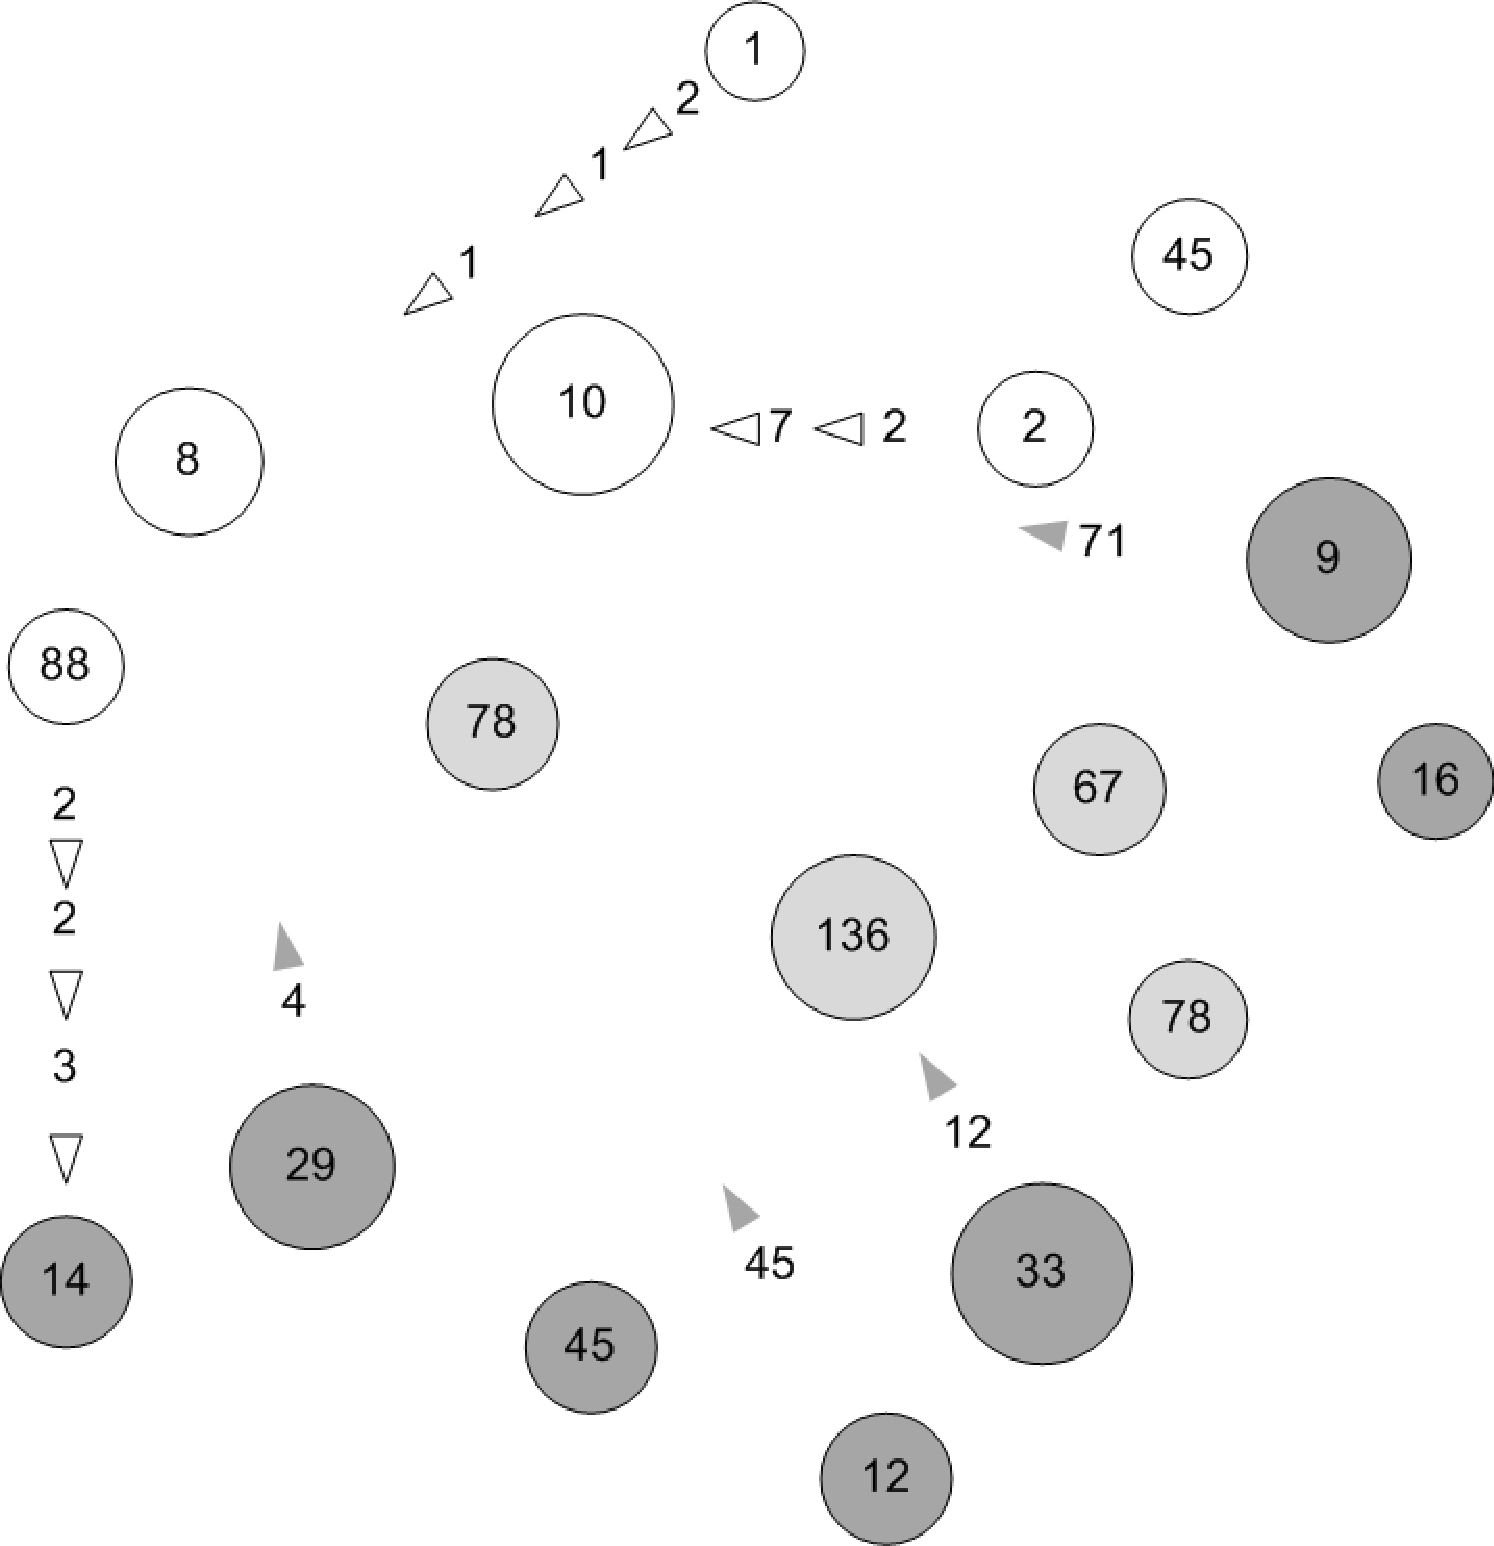
\epsfig{file=./imags/naves.pdf,width=7cm}
 \end{center}
 \caption{Simulated screenshot of an early stage of a run in Planet Wars. White planets belong to the player (blue colour in the game), dark grey belong to the opponent (red in the game), and light grey planets belong to no player. The triangles are fleets, and the numbers (in planets and triangles) represent the ships. The planet size means growth rate of the amount of ships in it (the bigger, the higher).}
 \label{figura:PlanetWars1}
 \end{figure}

A Planet Wars match takes place on a map (see Fig. \ref{figura:PlanetWars1})
that contains several planets (neutral, enemies, or own), each one of
them with a number assigned to it. This number represents the amount of ships
that the planet is currently hosting. 

The aim of the game is to destroy all the ships in planets owned by
the opponent. Although Planet Wars is a RTS game, this implementation
has transformed it into a turn-based game, in which each player has a
maximum number of turns to accomplish the objective. At the end of the
match, the winner is the player that remains alive, or that which owns
more ships if more than one survives.  

There are two strong constraints that determine the possible methods
to apply in order to design a bot that can play and win this game: the time for making a decision is \textit{just one second},  
and the bot is \textit{not allowed to store any kind of information}
about its former actions, about the opponent's actions or about the
state of the game (i.e., the game's map).  

Therefore, the objective of this paper is to generate a reliable DT
for a bot, which, according to the state of the map in every simulated
turn (input), returns a set of actions to perform in order to fight
the enemy, conquer its resources, and finally, win the game.  


%-----------------------------------------------------------------------
%%%%%%%%%%%%%%%%%%%%%%%% STATE OF THE ART %%%%%%%%%%%%%%%%%%%%%%%%%%%%%%
%-----------------------------------------------------------------------
\subsection{Related works}
\label{sec:soa}

RTS games have been used extensively in the Computational Intelligence (CI) area (see \cite{Lara2013review} for a survey). 
Among other techniques, EAs have been widely used as a CI method in RTS games, for example, for parameter optimisation \cite{Genebot_CEC11,ExpGenebot_CIG2012}, building order decision \cite{Kostler2013:MO_StarCraftII,Barriga2014:BuildingOrder_GA}, learning \cite{learning_StarCraft_AAIDE11,Wender_RL_CIG12}, or content generation \cite{Mahlmann2012MapGeneration,Lara_EntComp_PCG_RTS14}. 

GP has also proved to be a very good tool for developing strategies in
games, achieving results comparable to human, or human-based
competitors \cite{Sipper2007gameplaying}. They also have obtained
higher ranking than solvers produced by other techniques or even
beating expert human players \cite{Elyasaf2012FreeCell}. GP has also
been used in different kind of games, such as board-games
\cite{Benbassat2012Reversi}, (apparently) `simple' games like
Ms. Pac-Man \cite{Brandstetter2012PacMan} or Spoof
\cite{Wittkamp2007spoof}, and even in modern videogames such as First
Person Shooters (FPS) as Unreal\texttrademark~
\cite{Mora_UnrealBots10,Esparcia2013GPunreal}. 

In fact, GP has not been widely used in RTS games, so
there are just a few applications, such as pathfinding\footnote{http://www.gamasutra.com/view/feature/131147/evolving\_pathfinding\_algorithms\_.php?print=1}, definition of tactics in an abstract
tactical game \cite{KeaveneyO09_GP_RTS}, and recently to the automatic generation of strategies for a bot in StarCraft \cite{Garcia15Starcraft}.

This paper describes the application of a GP approach inside a `simple' RTS, Planet Wars, in order to define the whole behavioural engine for a bot. However, several approaches, based on three different fitness functions have been tested.
 
Planet Wars, the game used in this work, has also been used by other researchers
as an experimental framework for agent testing \cite{ZiolkoK12_PW_Reasoning} or for content generation \cite{Lara-CabreraCCL15}. 

We have worked on this game in some previous studies
\cite{Genebot_CEC11,genebot-evo12,Co-Genebot_EVO2014}, mainly applying
Genetic Algorithms for evolving (the parameters of) a behavioural
engine previously defined by a human expert from scratch.   

In the same line, we applied GP in a previous approach for Planet Wars bots
\cite{Garcia14Treedepth}. This was a further step after those works, which aimed to avoid the behavioural limitations that the initial bots had, since they used a static Finite State Machine, which just offers a
few degrees of improvement (namely a set of eight parameters). 
Thus, GP was applied to create `flexible' Decision Trees (DT) that the bots
used to decide on different courses of action during the game. 
The resulting bots were able to beat GENEBOT \cite{Genebot_CEC11}, our initial bot improved by means of GAs.

The present paper goes another step further and analyses the influence of different fitness functions on the algorithms performance and also on the generated individuals (bots). Usually, the score of a bots after a run is used \cite{StanleyBM05,LimBC10,ColeLM04}.

However, as it is usual when EAs are applied \cite{Jin2005303,QianYZ13}, and also due to the pseudo-stochastic nature of games, the evolution of bots is sensitive to {\em uncertainty} or {\em noise} \cite{merelo14:noisy}, even in a `simple' game as Planet Wars \cite{Mora_noisy_jcst}.
Basic strategies to handle noisy fitness functions include using a larger population size, averaging to filter out the noise (re-sampling) \cite{Branke98_robust}, thresholding (employing a threshold value to be used in a selection operator for noisy fitness functions) \cite{Markon2001_thresholding}, or changing the selection criteria.

Thus, in the paper we also propose testing the different fitness functions with the aim of checking which one if less sensitive to this kind of noise. This study will be useful to other researchers in order to select the best type of evaluation function, when defining other evolutionary methods working on RTSs.

The work also includes a study regarding the evolution of the generated Decision Trees along evolution, in order to show how do they change and how the conditions and actions are distributed on these trees. Moreover, this study lets us identify the type of strategies that the best bots follow, i.e. we can extract some {\em automatically generated knowledge} (or tips) that could help another bot designers or players to improve their skills in the game.


%-------------------------------------------------------------
%%%%%%%%%%%%%%%%%%%%%%%% GP BOT %%%%%%%%%%%%%%%%%%%%%%%%%%%%%%
%-------------------------------------------------------------
\section{GPBot}
\label{sec:agent}


The Genetic Programming-based bot or {\em GPBot} \cite{Garcia14Treedepth} evolves a set of rules which, in turn, models a Decision Tree (DT).

During the evolution, every individual in the population (a tree) must be evaluated. To do so, the tree is set as the behavioural engine of an agent, which is then placed in a map against a rival in a Planet Wars match. Depending on the obtained results, the agent (i.e. the individual) gets a fitness value, that will be considered in the evolutionary process as a measure of its validity. 
 
Thus, during the match the tree will be used (by the bot) in order to select the best strategy at every moment, i.e. for every planet a target will be selected along with the number of ships to send from one the other.

\noindent The used DTs are binary trees of expressions composed by two different \textit{types of nodes}:

\begin{itemize}
\item {\em Decision}: a logical expression formed by a variable, a less than operator ($<$), and a number between 0 and 1. It is the equivalent to a ``primitive'' in the field of GP.
\item {\em Action}: a leave of the tree (therefore, a ``terminal''). Each action is the name of the method to call from the planet that executes the tree. This method indicates to which planet send a percentage of available ships (from 0 to 1). 
\end{itemize}

The decisions are based on the values of different \textit{variables} which are computed as ratios considering all the available data in the game. For example, a possible variable is the ratio between the player ships and the enemy ones ({\em myShipsEnemyRatio}). Therefore, the decision \textit{myShipsEnemyRatio $<$ 0.5} will trigger a \textit{true} if we have less ships than the enemy. All the possible variables are summarized in Table \ref{tab:decisions}.


\begin{table}
\resizebox{12cm}{!}{
\begin{tabular}{|l|p{4cm}|p{4cm}|}
\hline
{\em Name} & {\em Numerator} & {\em Denominator} \\ \hline \hline
 myShipsEnemyRatio 			&  player's ships & enemy's ships \\ \hline
 myShipsLandedFlyingRatio   &  player's landed & flying ships \\ \hline
 myPlanetsEnemyRatio 		&  number of player's planets & the enemy's ones \\ \hline
 myPlanetsTotalRatio 		&  number of player's planet & total planets (neutrals and enemy included) \\ \hline
 actualMyShipsRatio 		&  number of ships in the specific planet that evaluates the tree & player's total ships \\ \hline
 actualLandedFlyingRatio 	&  number of ships landed and flying from the specific planet that evaluates the tree & player's total ships \\ \hline
\end{tabular}
}
\caption{Possible decisions in a generated tree.}
\label{tab:decisions}
\end{table}

Finally, the possible \textit{actions} are listed in Table \ref{tab:actions}. Every action sends ships to an objective planet. These planets can be the enemy's, neutral, any of them, or the player ones. For example, the action \textit{AttackNearestNotMyPlanet(0.7)} will send the 70\% of the ships in the planet that executes the tree, to the nearest planet (enemy or neutral).

\begin{table}
\resizebox{12cm}{!}{
\begin{tabular}{|p{5cm}|p{8cm}|}
\hline
{\em Name} & {\em Action} \\ \hline \hline
AttackNearestNeutralPlanet \newline AttackNearestEnemyPlanet \newline AttackNearestNotMyPlanet & The objective is the nearest (neutral, enemy or either) planet \\ \hline
AttackWeakestNeutralPlanet \newline AttackWeakestEnemyPlanet \newline AttackWeakestNotMyPlanet & The objective is the (neutral, enemy or either) planet with less ships \\ \hline
AttackWealthiestNeutralPlanet \newline AttackWealthiestEnemyPlanet \newline AttackWealthiestPlanet & The objective is the planet (enemy, neutral or either) with higher growth rate \\ \hline
AttackBeneficialNeutralPlanet \newline AttackBeneficialEnemyPlanet \newline AttackBeneficialPlanet & The objective is the  more beneficial planet, that is, the one with highest growth rate divided by the number of ships \\ \hline
AttackQuickiestNeutralPlanet \newline AttackQuickiestEnemyPlanet \newline AttackQuickiestPlanet & The objective is the planet easier to be conquered: the lowest product between the distance from the planet that executes the tree and the number of  ships in the objective planet \\ \hline
AttackNearestNeutralBase \newline AttackNearestEnemyBase \newline AttackNearestNotMyBase & The objective is the planet (neutral, enemy or either) with more ships (that is, the base) \\ \hline
 Attack Random Planet & Send ships to a random enemy or neutral planet\\ \hline
Reinforce Nearest Planet & Reinforce the nearest player's planet to the planet that executes the tree \\ \hline
Reinforce Base & Reinforce the player's planet with higher number of ships \\ \hline
Reinforce Wealthiest Planet & Reinforce the player's planet with higher grown rate \\ \hline
Do nothing & \\ \hline
\end{tabular}
}
\caption{Possible actions in a generated tree. For example, the action \textit{AttackNearestNotMyPlanet(0.7)} will send the 70\% of the ships in the planet that executes the tree, to the nearest planet (enemy or neutral).}
\label{tab:actions}
\end{table}



\noindent An example of a possible DT is shown in Figure \ref{fig:sourcecode}. The example tree
shown below has a total of 5 nodes, with 2 decisions and 3 actions, and a
depth of 3 levels. 

\begin{figure}

\begin{Verbatim}[frame=single]

if(myShipsLandedFlyingRatio < 0.796)
   if(actualMyShipsRatio < 0.201)
      attackWeakestNeutralPlanet(0.481);
   else
      attackNearestEnemyPlanet(0.913);
else
   attackNearestEnemyPlanet(0.819);

\end{Verbatim}

\caption{Example of the generated source of a DT obtained by the algorithm.}
\label{fig:sourcecode}
\end{figure}

\noindent The bot's behaviour is explained in Algorithm \ref{alg:turn}.

\begin{algorithm}[ht]
\begin{algorithmic}

\STATE // At the beginning of the execution the agent receives the tree
\STATE tree $\leftarrow$ readTree()
\WHILE{game not finished}
	\STATE // starts the turn
	\STATE calculateGlobalPlanets() // e.g. Base or Enemy Base
	\STATE calculateGlobalRatios() // e.g. myPlanetsEnemyRatio
	\FOR{Each p in PlayerPlanets}
		\STATE calculateLocalPlanets(p) // e.g. NearestNeutralPlanet to p
		\STATE calculateLocalRatios(p) //e.g actualMyShipsRatio
		\STATE executeTree(p,tree)  // Send a percentage of ships to destination
   \ENDFOR
\ENDWHILE

\end{algorithmic}
\caption{Pseudocode of the proposed agent. The same tree is used during all the agent's execution}
\label{alg:turn}
\end{algorithm}


Next section explains the three different fitness functions that have been implemented to evaluate the agents' performance during the battles. 


%-----------------------------------------------------------------------
%%%%%%%%%%%%%%%%%%%%%%%% FITNESS FUNCTIONS %%%%%%%%%%%%%%%%%%%%%%%%%%%%%
%-----------------------------------------------------------------------

\section{Fitness Functions}
\label{sec:fitness_functions}

% ---------------------------------------------------------------------

Fitness function should have some characteristics in order to ensure a good performance of the algorithm where it is used: 
\begin{itemize}
\item to create a smooth landscape: yield close values in the evaluation of close/similar individuals.
\item being readily available: every correct individual can always be evaluated.
\item being robust: the evaluation of a specific individual should be always the same (or similar, at least).
\item being reliable: a good individual (according to the problem objective) must get a higher fitness value than a bad one.
\end{itemize}

This section describes three different fitness functions to be applied in the GP algorithm described in Section \ref{sec:agent}, in order to generate competitive bots for Planet Wars.

Thus, Subsection \ref{subsec:fitness_turns} presents a hierarchical fitness based on the number of victories, and also the number of turns of the battles for tiebreaks. This function is an evolution of the one we used in previous works \cite{Genebot_CEC11,genebot-evo12,Garcia14Treedepth}.
Subsections \ref{subsec:fitness_slope} and \ref{subsec:fitness_area} show two other fitness functions which take into account the behaviour of the agents during the battles, i.e. they consider the percentage of resources (ships) gathered by the bot, and compute, respectively, a slope or an area as its evaluation value. These are also the improvement (and adaptation to this GP approach) of previous proposals \cite{Co-Genebot_EVO2014}. They aim to evaluate other factors of the battle, rather than just consider if the bots win or lose. 
Thus, we finally want to analyse in the work if these factors are important in order to evolve enough competitive bots.


% ---------------------------------------------

\subsection{Fitness based on Victories}
\label{subsec:fitness_turns}

The justification of this fitness is to reach the main objective we pursuit with this method: generate bots able to win as many times as possible.
This is an improvement of the hierarchical fitness considered in \cite{Genebot_CEC11}.
In this approach, an individual is better than another if it wins in a larger number of maps. In case of equality of victories, then the individual with more turns to be defeated (i.e. the stronger one) is considered as better. 
Every evaluation consists in five battles against the same enemy, GENEBOT
 \cite{Genebot_CEC11}, so the maximum fitness value with this approach is 5 victories and 0 turns. 
For two bots, A and B, the fitness comparison (and therefore, their order inside the population) is defined as Algorithm \ref{alg:fitness_turns_positions} shows.

\begin{algorithm}[ht]
\begin{algorithmic}
        
\STATE $A,B \in Population$
\IF{A.victories $=$ B.victories}
	\IF{A.turns $>=$ B.turns}
		\STATE A is better than B
	\ELSE
		\STATE B is better than A
	\ENDIF
\ELSE
	\IF{A.victories $>$ B.victories}
		\STATE A is better than B
	\ELSE
		\STATE B is better than A
	\ENDIF
\ENDIF

\end{algorithmic}
\caption{Comparison between two individuals using fitness based on victories}
\label{alg:fitness_turns_positions}
\end{algorithm}

In this fitness, we are only interested in the final result of the battles (position and number of turns). We do not include in the computation how the bot has reached them. The problem of this function is that the consideration of two different terms (victories and turns) makes it difficult the comparison between different evaluations, and it is hard to decide which individual is better if both have won just some of the battles. 

Thus, in this work, two additional evaluation functions have been proposed in order to make a, in principle, fairer comparison between bots, trying to add another factor in order to be less sensitive to noise \cite{Mora_noisy_jcst}. 
Both of them are based on the percentage of ships belonging to each player in every turn. They are normalised considering the total amount of ships in the game for that turn (including neutral ships in neutral planets), so for each player, there is a different {\em cloud of ships}.
In the next subsections there are described the two alternatives to transform this cloud of points into a singular value for the fitness function: the use of slopes (statistical method) and areas (numerical method).

% ---------------------------------------------------------------------

\subsection{Fitness based on Slope}
\label{subsec:fitness_slope}

In this case, a square regression analysis is computed in order to transform the cloud of points into a simple line. The line is represented as {$y = \alpha \times x + \beta $}, where {$\alpha$} and {$\beta$} are calculated as shown in Equations \ref{eq:alpha} and \ref{eq:beta}, computing a least squares regression. For every bot in the simulation we calculate $\alpha$ and ($slope$). This $slope$ is the fitness of every bot for that simulation. 

\begin{equation}
\label{eq:alpha}
        \alpha = \frac{\sum_{i=1}^{n}(X_{i} - \bar{X_{i}})(Y_{i} - \bar{Y_{i}})}{\sum_{i=1}^{n}(X_{i} - \bar{X_{i}})^{2}}
\end{equation}

\begin{equation}
\label{eq:beta}
        \beta = \bar{Y}-\alpha\bar{X}
\end{equation}

Theoretical maximum and minimum values are set for this fitness. An optimum bot that wins in the first turn, has an ideal slope of {$1$}, so this is the maximum value of our fitness. On the other hand, a bot that loses in the first turn,  has a slope of {$-1$}. Thus, if we calculate the $slope$, we know if the bot {$WINs$} ({$slope>0$}) or {$LOSEs$} {$slope<0$}. 
The values of the five different battles are summed to compute the global $slope$. Then, the bot with the highest value will be the best is each simulation or battle. 

This method, theoretically, assigns the fairest value to an individual, since the obtained result is highly correlated to the victory or lose in the battle, being it positive or negative, respectively. Moreover, the value will be higher if the number of resources/ships gathered has been higher, and the other way round. 


% ---------------------------------------------------------------------

\subsection{Fitness based on Area}
\label{subsec:fitness_area}

In this function, the integral of the curve of the bot's live-line is used for calculating the area that is `covered' by the fitness cloud of points (see Equation \ref{eq:area}). This {$area$} is normalised considering the number of turns, and thus it represents the average percentage of owned ships during the battle for each player. 

\begin{equation}
        area=\frac{\int_{0}^{t}\%ships(x)dx}{t}
    \label{eq:area}
\end{equation}

As in previous case, maximum and minimum values have been set for this fitness. If an optimal bot wins in the first turn, the area of each live-line is close to {$1$}, so this is the maximum value of the fitness. Otherwise, if a bot loses in the first turn, its live-line area is close to {$0$}. 

In this case, we do not extract additional information about which bot wins the battle, because the area of the live-line is not related with the winner of the battle. Thus, some information is lost. 

However, in spite of the missed information, this method is better than slope in order to differentiate between bots which have an intermediate value for the hierarchical fitness. Thus, the assigned value with this function is useful to decide if it is better a bot which wins sometimes, but when it loses, the match last just a few turns; or a bot which loses many times, but the matches takes a large number of turns.


%-----------------------------------------------------------------------
%%%%%%%%%%%%%%%%%%%%%%%%%%%% EXPERIMENTS %%%%%%%%%%%%%%%%%%%%%%%%%%%%%%%
%-----------------------------------------------------------------------

\section{Experiments and results}
\label{sec:experiments}

In this section we first describe and justify the considered operators and parameter values. Then the experiments are conducted and the obtained results are analysed.

\subsection{Algorithm configuration}
\label{subsec:alg_config}

The GP algorithm has been configured using standard operators, as other researchers proposed in similar implementations \cite{Esparcia2013GPunreal}. Thus, a \textit{sub-tree crossover} has been applied, which chooses one node in every parent tree and interchanges the whole sub-trees below them. In addition a \textit{1-node mutation} has been considered. Thus, the mutation randomly changes the action or the value of a leaf node with a mutation rate of 0.25 (an adequate value empirically tested). 
The population is formed by 32 individuals and the \textit{2-tournament selection mechanism} has been applied to select the parents of the new offspring in every generation of the algorithm. So, two parents are chosen from a pool of 16 and they compete each other to be the winner. The process is repeated for selecting another parent and both generate a couple of new individuals which will then substitute the two worse in the current population, following an \textit{steady-state replacement policy} (most of the individuals in the population remain from one generation to the next). 
To \textit{evaluate} every individual during the evolution, a battle with a previously created bot is performed in 5 different (but representative) maps provided by Google, computing a fitness value according to the proposed functions. 

Also, and due to the presence of noise (different evaluations will yield different values), all individuals are re-evaluated in every generation, constituting an implicit averaging as it is suggested by the authors in \cite{Jin2005303,DBLP:conf/ijcci/MereloLFGCCRMG15}.

A publicly available bot has been chosen for the
experiments\footnote{It can be downloaded from \url{https://github.com/deantares/genebot}}. 
The bot to confront is {\em GENEBOT}, proposed in \cite{Genebot_CEC11}. As stated, this bot was trained using a GA to optimise the eight parameters that conforms a set of hand-made rules, obtained from the experience of an expert human player. Table \ref{tab:parameters} shows the values of the parameters considered.

\begin{table}
\begin{center}
\begin{tabular}{|c|c|}
\hline
{\em Parameter Name} & {\em Value} \\\hline \hline
Population size & 32 \\\hline
Crossover type & Sub-tree crossover \\ \hline
Crossover rate & 0.5\\ \hline
Mutation  & 1-node mutation\\ \hline
Mutation step-size & 0.25 \\ \hline
Selection & 2-tournament \\ \hline
Replacement & Steady-state\\ \hline
Stop criterion & 50 generations \\ \hline
Maximum Tree Depth & 7  \\ \hline 
Runs per configuration & 30 \\ \hline
Evaluation & Playing versus GENEBOT \cite{Genebot_CEC11}  \\ \hline 
Maps used for evaluation & map76, map69, map7, map11, map26 
\\ \hline
\end{tabular}
\caption{Parameters used in the experiments}
\label{tab:parameters}
\end{center}
\end{table}

Each configuration is executed 21 times in order to obtain statistically significant results.
After all the executions we have evaluated the obtained best individuals in all runs confronting to the other bots in a larger set of maps, 

in order to study the behaviour of the algorithm and how good are the obtained bots versus enemies and maps that have not been used for training.

The algorithm has been implemented using OSGiLiath, a service-oriented evolutionary framework \cite{Garcia13Service}. 
The generated tree is compiled in real-time and injected in the agent's code using Javassist \footnote{\url{www.javassist.org}} library. All the source code used in this work is available under a LGPL V3 License in \url{http://www.osgiliath.org}.



%-------------------------------------------------------------
%%%%%%%%%%%%%%%%%%%%%%%% RESULTS %%%%%%%%%%%%%%%%%%%%%%%%%%%%%
%-------------------------------------------------------------
\subsection{Analysis of Results}
\label{subsec:results}

This section presents several analyses firstly (in the following subsection)  focused on the algorithmic process and on the evolution of the individuals and their fitness values, also taking into account the influence of noise. Second (in Subsection \ref{subsubsec:fitness_benchmark}, an analysis has been conducted considering the best individuals obtained by every approach, testing them against other opponents from the literature and in combats among themselves.

\subsubsection{Study of the GP algorithm and Fitness Functions}
\label{subsubsec:evolutionary_algorithm}

Table \ref{tab:results3config} shows the obtained results after
executing each approach (GP + fitness function) 21 times. 
Although the fitness are not comparable, as they obviously apply different metrics, the \textit{Victory}-based fitness achieves values near to the optimum (5) at the end of the run (look at the best individual and average population values). The \textit{Area}-based and \textit{Slope}-based fitness yield results under their theoretical optimum, as they depend on more information ranges (variation in the number of ships). 

\begin{table*}
\centering{
\begin{tabular}{|c|c|c|} \hline            
		& Average best fitness	&	Average population fitness	\\ \hline \hline
Victory	& 4.761 $\pm$	0.624	&	4.345	$\pm$	0.78 \\ \hline
Area	& 2.838	$\pm$	1.198	&	2.347	$\pm$	0.949 \\ \hline
Slope	& 2.296	$\pm$	0.486	&	2.103	$\pm$	0.434 \\ \hline

\end{tabular}
\caption{Average results obtained for each approach at the end of the 21
  runs}
\label{tab:results3config}
}
\end{table*}

However, in the three following figures we have conducted a graphical study of the evolution of fitness on the runs in order to present a kind of visual comparison.
Figure \ref{figura:fitness_turns} shows how the fitness of the best individuals and also the average fitness of the population are improved along generations, as it is desired in an EA. Figures \ref{figura:fitness_area} and \ref{figura:fitness_slope} show the same tendencies. Moreover, as expected, the fitness of the best individuals has a higher progression than averages.
These facts mean that the fitness functions are correctly defined and are properly working.

Comparing the results for every fitness with the rest, it can be seen that Victory fitness shows a higher progression than the others. This is due to the range of the dominions of values in these functions. However, it can be noted that the variability of values is higher in Area than in Slope, because of the negative values that can be yielded in the latter.
% Antonio - es por esto? Que estoy medio dormido. :(

As it can be seen in the dispersion of the cloud of points, the \textit{noise} is present in all the functions, but \textit{Area shows a better tolerance} to it, since the cloud is a bit narrower than the others.


\begin{figure}[ht]
 \begin{center}
 \makebox[\linewidth][c]{
   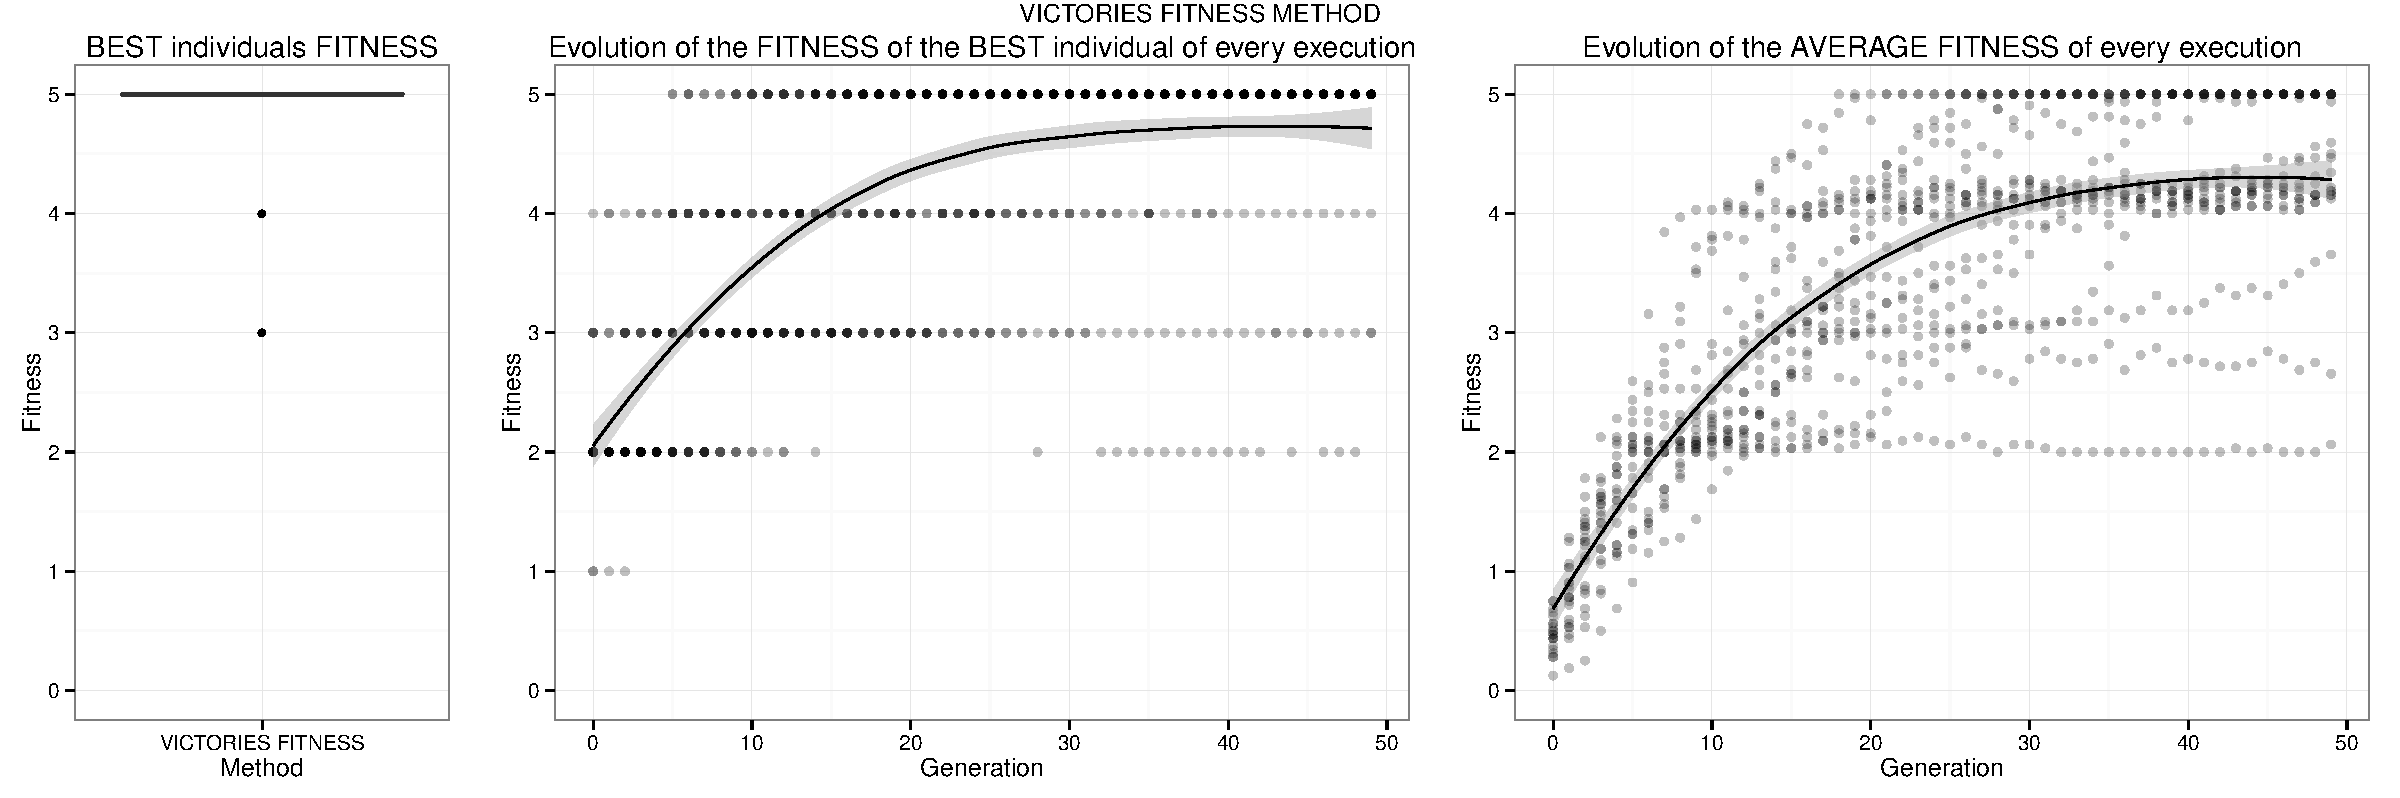
\includegraphics[width=15cm]{nuevas_imgs/estudio_turns.pdf}
   }
 \end{center} 
 \caption{\textbf{Victory-based Fitness} individuals: Boxplot of the fitness of the \emph{Best individuals}, one per run, and evolution of the \emph{Best fitness} and \emph{Average population fitness} of every execution. In the evolution plots (centre and right), single points and locally weighted polynomial curve (loess) are shown.}
 \label{figura:fitness_turns}
 \end{figure}

   \begin{figure}[ht]
 \begin{center}
 \makebox[\linewidth][c]{
   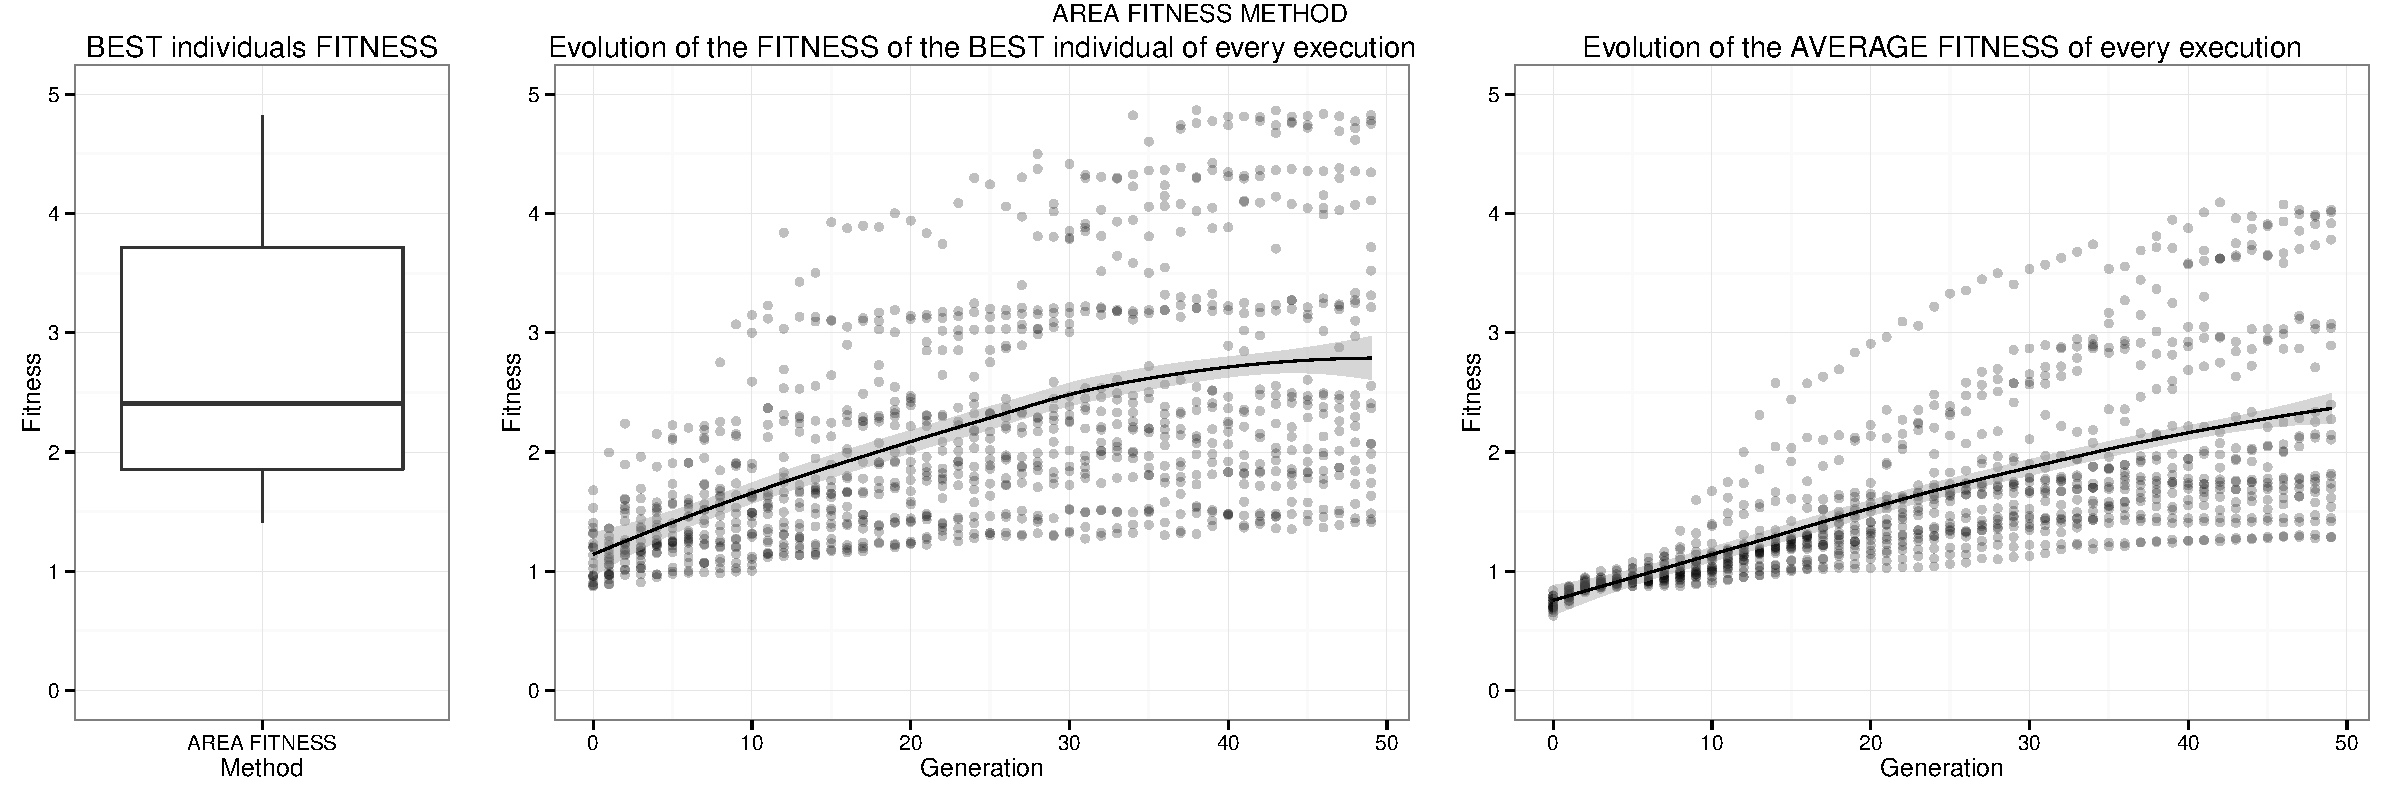
\includegraphics[width=15cm]{nuevas_imgs/estudio_area.pdf}
   }
 \end{center}
 \caption{\textbf{Area-based Fitness} individuals: Boxplot of the fitness of the \emph{Best individuals} of every execution and evolution of the \emph{Best fitness} and \emph{Average population fitness} of every execution. In evolution plots (centre and right), single points and locally weighted polynomial curve (loess) are shown.}
 \label{figura:fitness_area}
 \end{figure}

    \begin{figure}[ht]
 \begin{center}
 \makebox[\linewidth][c]{
   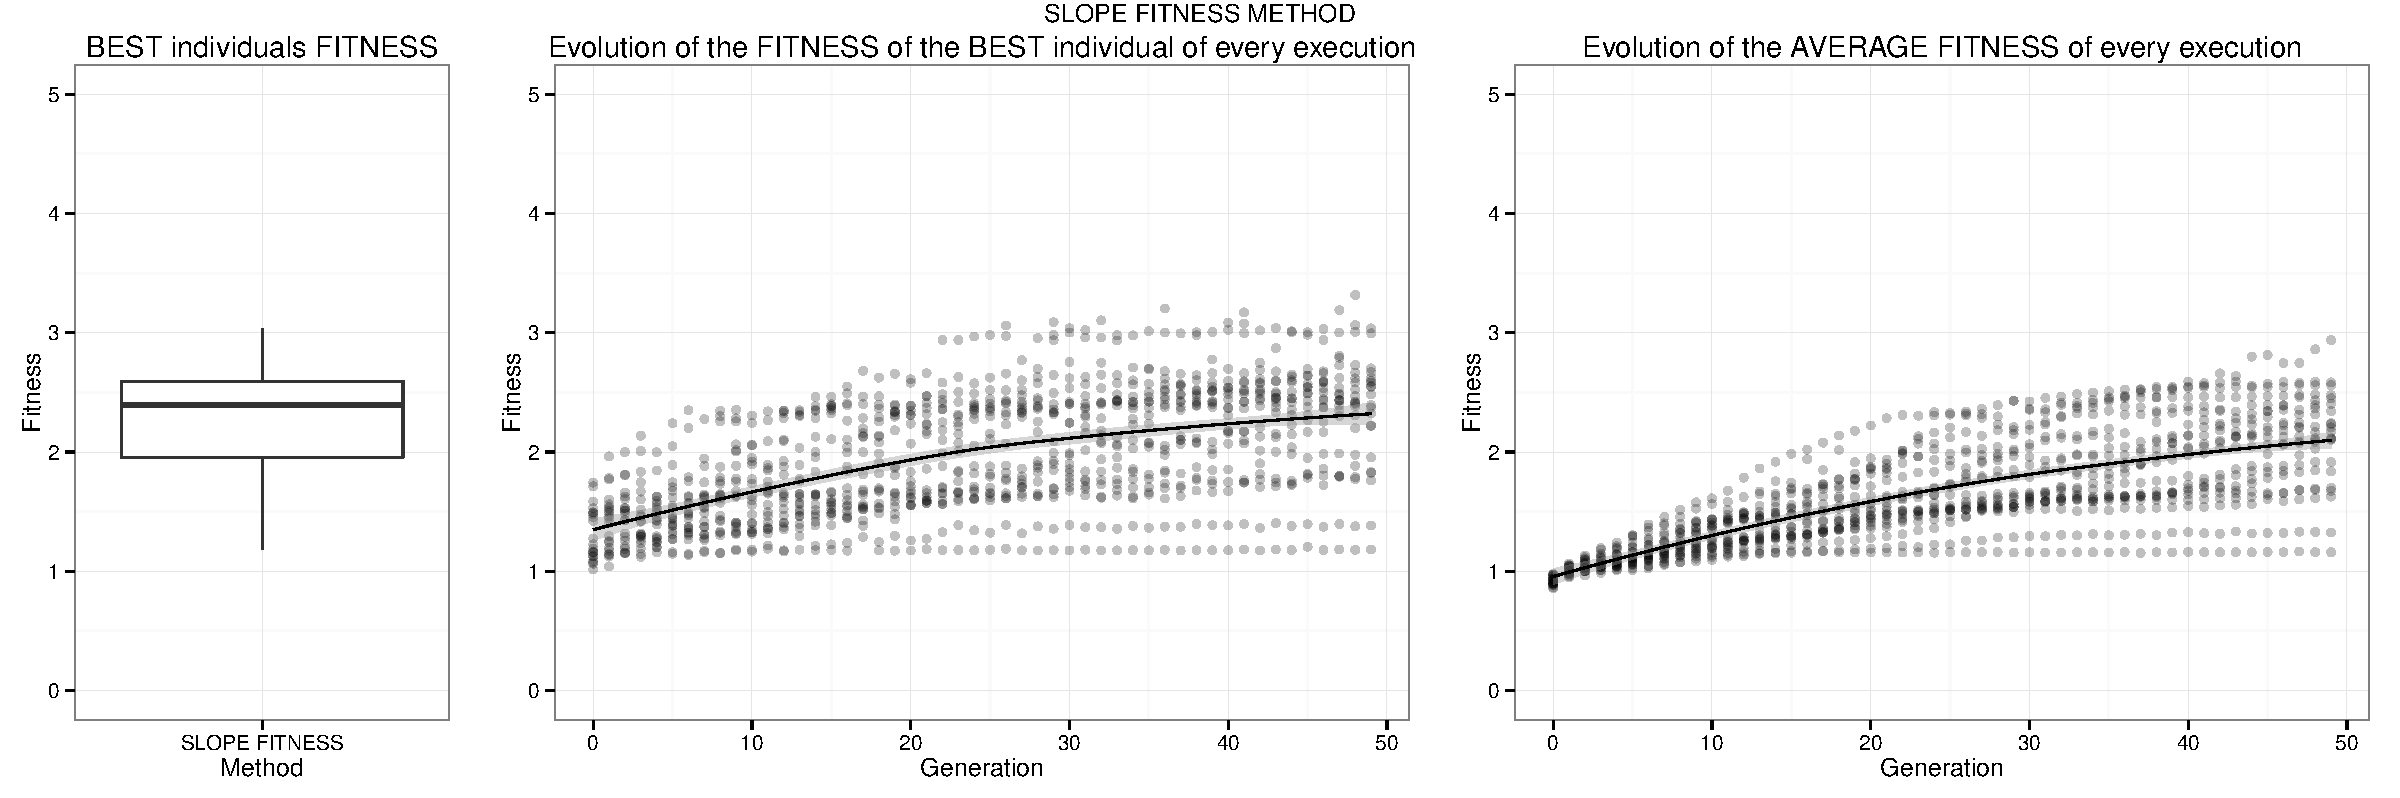
\includegraphics[width=15cm]{nuevas_imgs/estudio_slope.pdf}
   }
 \end{center}
 \caption{\textbf{Slope-based Fitness} individuals: Boxplot of the fitness of the \emph{Best individuals} of every execution and evolution of the \emph{Best fitness} and \emph{Average population fitness} of every execution. In evolution plots (centre and right), single points and locally weighted polynomial curve (loess) are shown.}
 \label{figura:fitness_slope}
 \end{figure}



Looking at the evolution of individuals (trees), Figure \ref{figura:evolutionDEPTH} shows the average depth of the trees along the 
The three approaches show a similar behaviour in this respect, i.e. the average depth grows in every generation. Victory fitness approach is the one with a smaller growing. Thus, it obtains smaller trees that are very good individuals anyway.

 \begin{figure}[ht]
 \begin{center}
 \makebox[\linewidth][c]{
   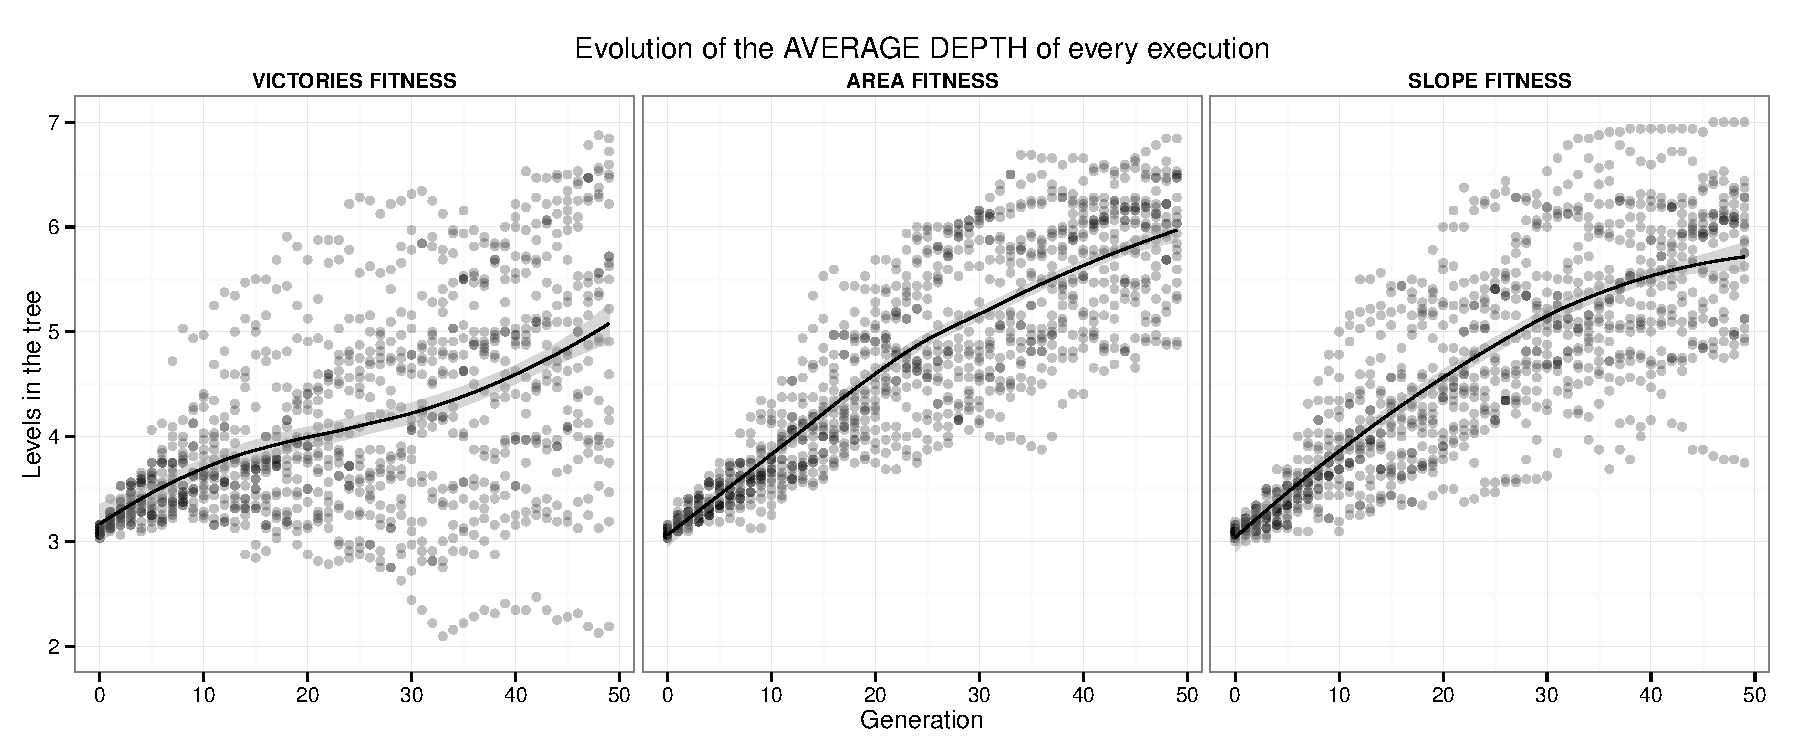
\includegraphics[width=15cm]{nuevas_imgs/evolution_AVERAGE_DEPTH.pdf}
   }
 \end{center}
 \caption{Evolution of the average depth of every run by fitness
   method}
 \label{figura:evolutionDEPTH}
 \end{figure}

Figure \ref{figura:evolutionAGE} plots the average age of the individuals in the population, i.e. the number of generations they survive. A constant growth in this graph will mean that the individuals are growing in age, so they are not being replaced, and the population is not being improved properly.
In the graphs we cannot appreciate a growing tendency after generation 10 for Victory and Slope, which means these functions a working well. However, Area behaves a bit different and a slightly progression is presented. This is another evidence that this method is \textit{less sensitive to noise}, and good individuals continue being good along generations. 


 \begin{figure}[ht]
 \begin{center}
 \makebox[\linewidth][c]{
   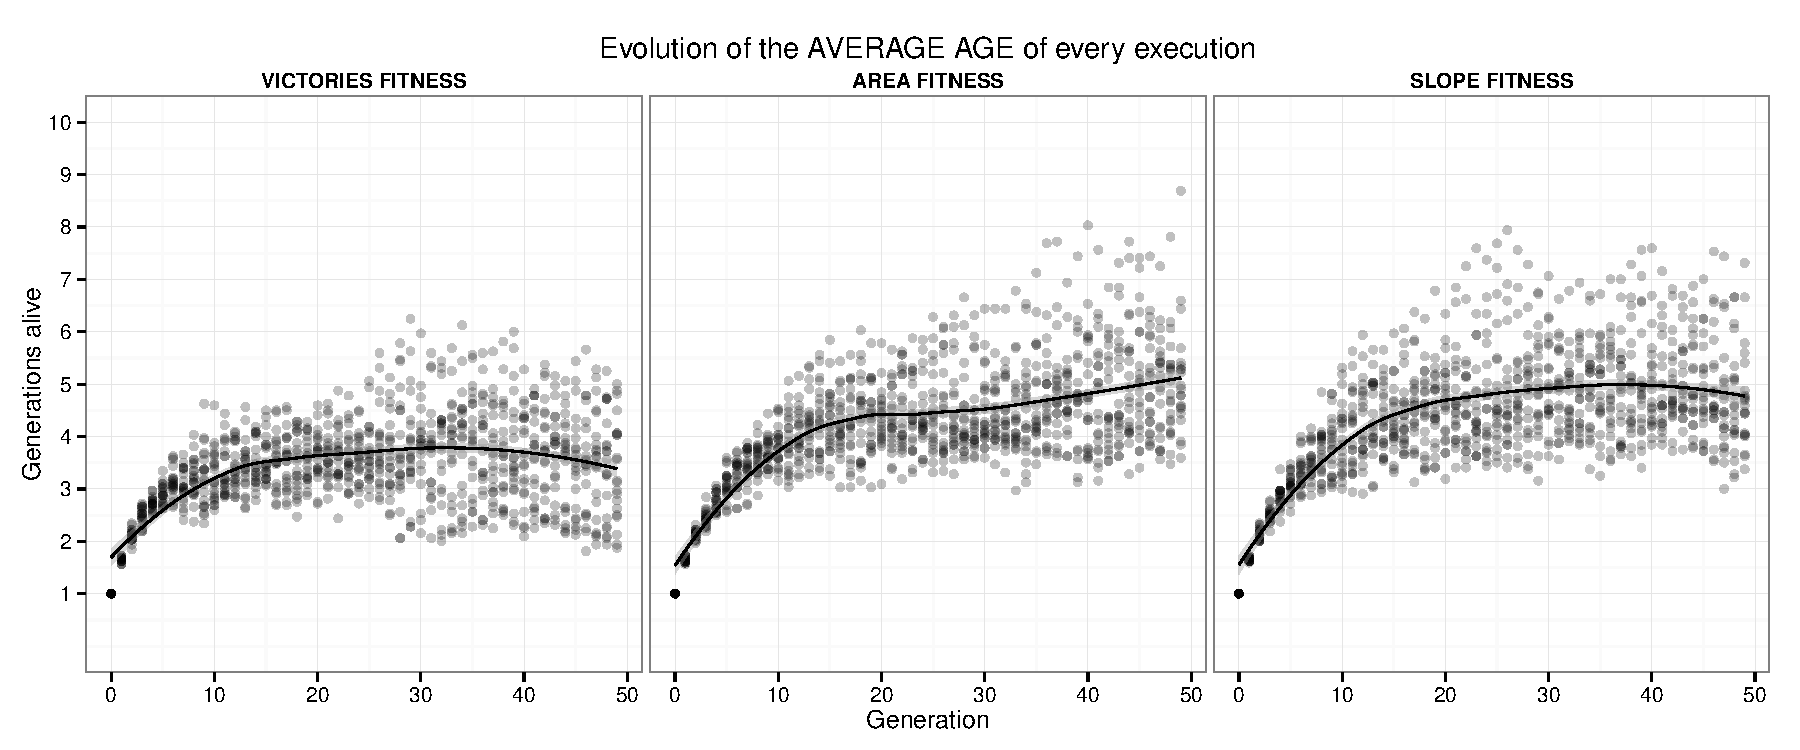
\includegraphics[width=15cm]{nuevas_imgs/evolution_AVERAGE_AGE.pdf}
   }
 \end{center}
 \caption{Evolution of the average age of the population in every run by fitness
   method} 
 \label{figura:evolutionAGE}
 \end{figure}


% -----------------------------------------------------------

\subsubsection{Fitness Benchmark}
\label{subsubsec:fitness_benchmark}

Even though the Victory-based fitness yields better results
(near optimal), to do a fair comparison, we have confronted the 21
best bots obtained with each configuration (one per run) against
EXPGENEBOT. However, these battles have been performed in 9 maps that were
different to the ones used to evolve the bots. These maps, provided by Google, are considered as representative \cite{ExpGenebot_CIG2012}, because they have different features to promote a wide set of strategies, i.e. different distributions of planets, sizes and number of initial ships. 

This experiment has been conducted in order to validate if the bots obtained by the proposed approaches can be competitive in terms of quality in maps not used for evolution/evaluation. Results are shown in Figure \ref{figura:boxplotvictoriesgenebot}. As it can be seen, the Victory-based fitness achieves significantly better results than the other methods.
This could be explained considering the way the fitness is computed, because Victory fitness tends to promote to its generated bots, obviously, just obtaining the victory. Area and Slope also take care of the number of ships generated during the battles, which may lead to a more `conservative' (less aggressive) behaviour. This would be tested in Section \ref{sec:analysis_DT}.

\begin{figure}[ht]
 \begin{center}
 \makebox[\linewidth][c]{
   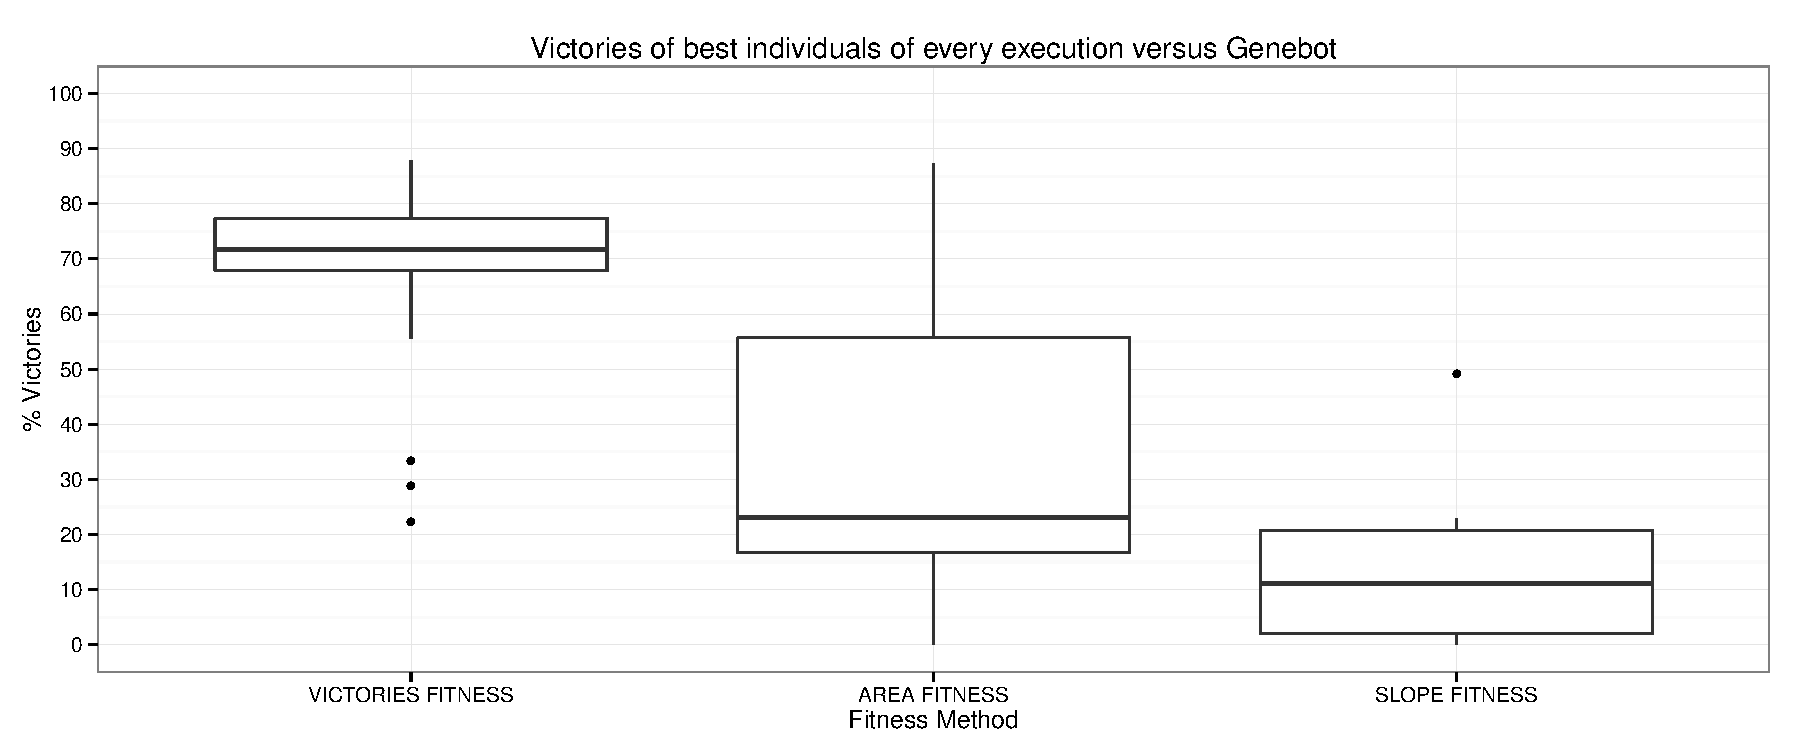
\includegraphics[width=15cm]{nuevas_imgs/vsGENEBOT_Boxplot.pdf}
   }
 \end{center}
 \caption{Boxplot of percentage of victories of the bots obtained by each approach vs EXPGENEBOT. 9 different battles have been performed per bot in different maps.} 
 \label{figura:boxplotvictoriesgenebot}
 \end{figure}

In order to complement these results an additional experiment has been conducted, making a direct comparison between the three methods. To this end, each one of the 21 best individuals obtained per approach has been tested competing against all the rest (in a 1 vs 1 battle) in 9 matches per pair of bots, one per representative map.

This allows a comparison with a bigger number of bots, and also,
allows the analysis of their behaviour against rivals not previously
used during training (as in the experiment above). 

The boxplots of the percentage of victories from the best bots
obtained by each method are shown in Figure
\ref{figura:boxplotvictories}. It is clear from the image that the
Slope fitness does not get good results compared with the other methods. This could happen due to this approach is \textit{the most sensitive to noise}, so, maybe the best individuals generated are not actually so good.

The Victory-based fitness achieves better results in average, being also more robust (small standard deviation). However, looking at the Area fitness results, they outperform several times the Victory results, obtaining more victories.


 \begin{figure}[ht]
 \begin{center}
 \makebox[\linewidth][c]{
   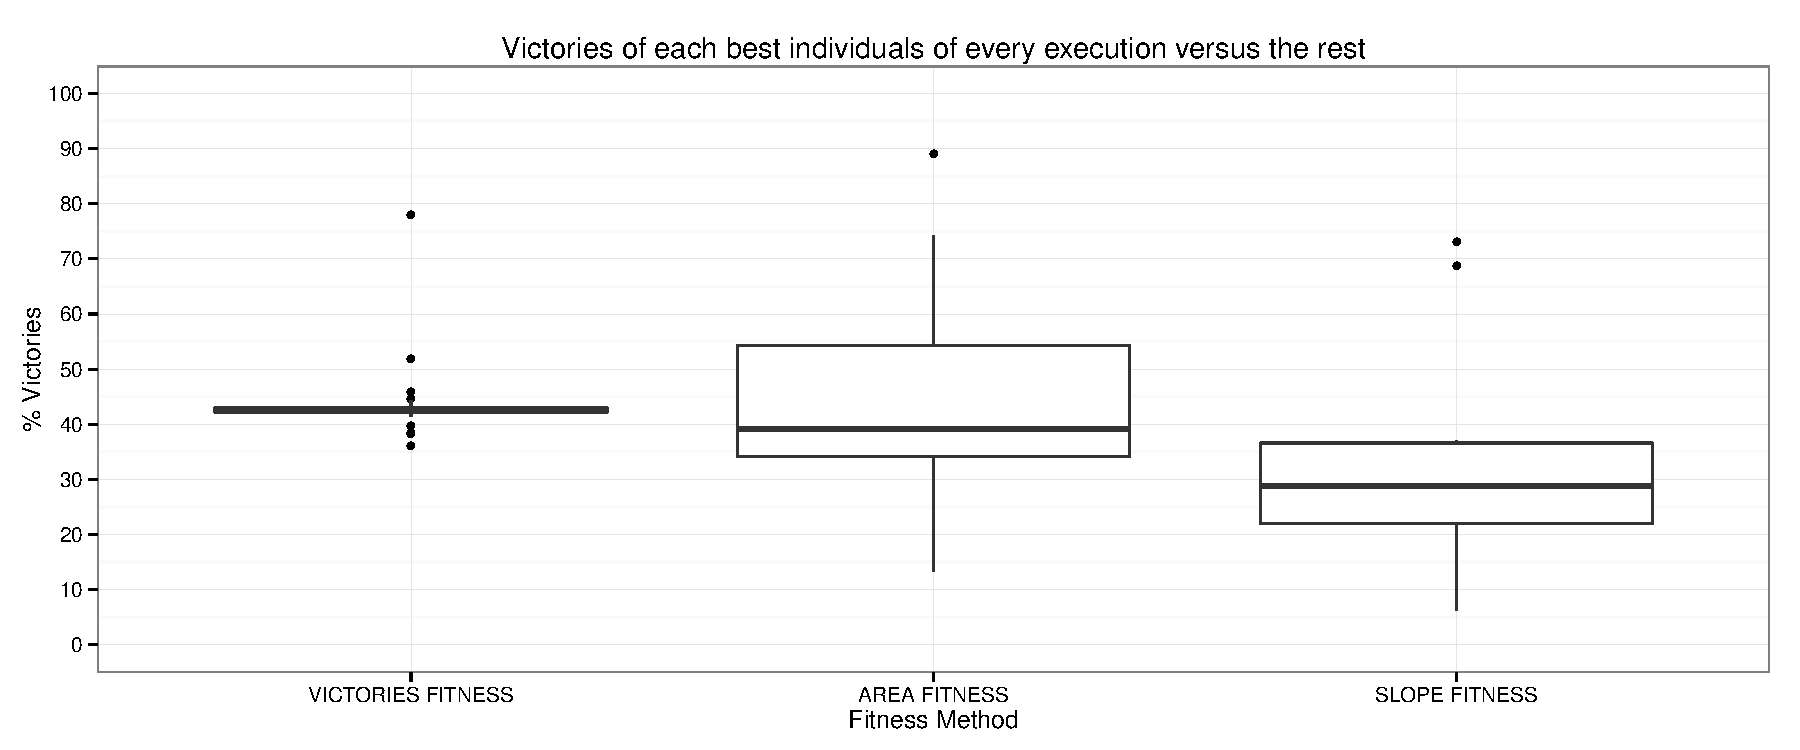
\includegraphics[width=15cm]{nuevas_imgs/batallas_Boxplot.pdf}
   }
 \end{center}
 \caption{Boxplot of the average percentage of victories of the best bots obtained by each method vs. the rest.}

 \label{figura:boxplotvictories}
 \end{figure}


%--------------------------------------------------------

\section{Analysis of obtained Decision Trees}
\label{sec:analysis_DT}

In this section, we present a complementary study on the distribution and appearance of the decisions and actions described in Section \ref{sec:agent}. This could allow to detect which elements that model the behaviour of the bots are more important during the game process, analysing the number of actions and decisions, and comparing their rate using the different compared fitness functions. This information can be useful to redefine the information used during the evolutionary process, such as the conditions and actions defined by the expert themselves, if they are not useful, according to this study. 

The analysis has been conducted on the best individuals obtained in
each generation for the three fitness methods, counting the percentage
of use of a decision/action in relation with the total of the same
type and taking into account all the best individuals of that
generation. Therefore, a more useful node to win the match will occur
with more frequency  in the best individuals during the algorithm run, and
vice versa. 

Figure \ref{figura:e_number_nodes} shows the average growing of
conditions and actions during the evolution. As described before in
Figure \ref{figura:evolutionDEPTH}, when the number of generations
increases, the depth also does, as well as, obviously, the number of
nodes. But in this case, in the latter generations of the Victory
fitness the number of nodes increases more than in the other two
fitness methods, being the depth of this method also lower than the
Slope and Area. This indicates that the Victory Fitness is generating
more balanced trees than the other methods. 

  \begin{figure}[ht]
  \begin{center}
  \makebox[\linewidth][c]{
    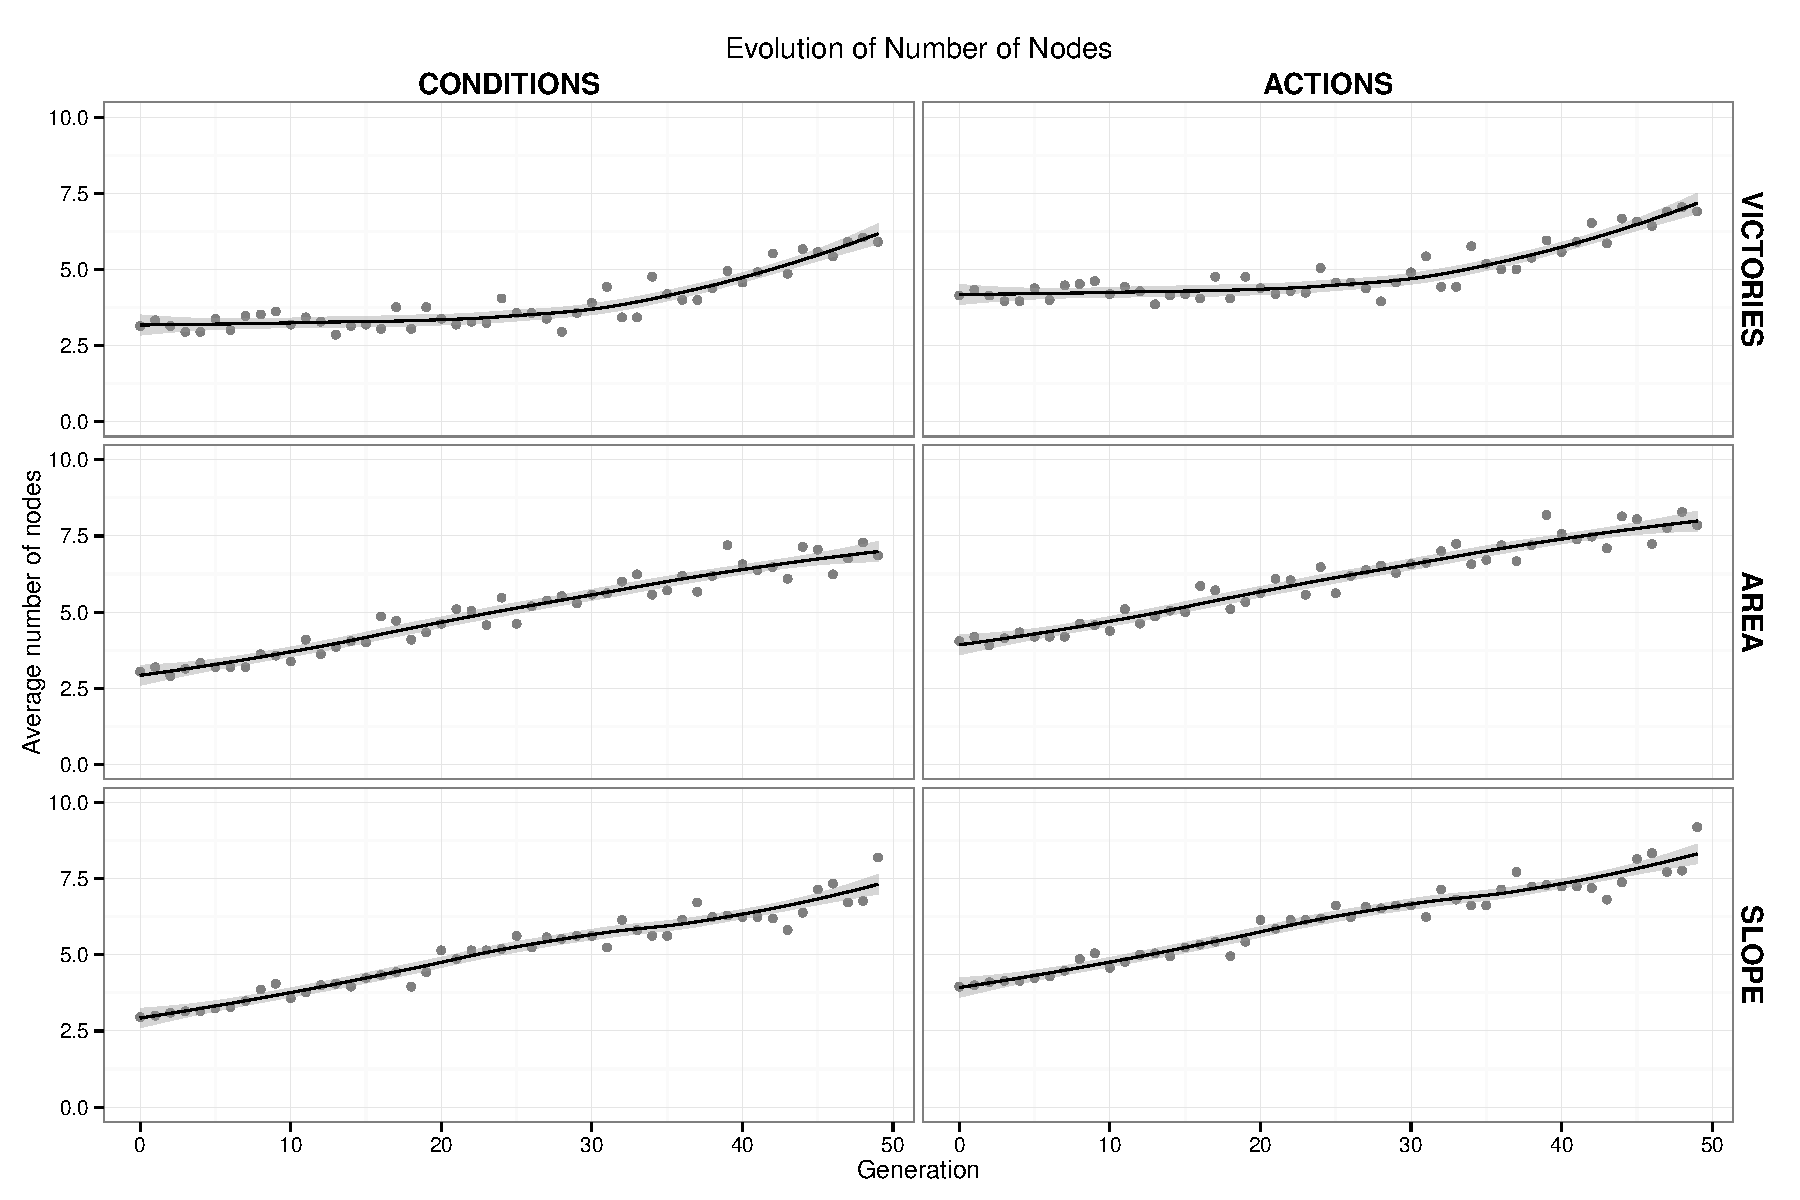
\includegraphics[width=15cm]{nuevas_imgs/estudio_number_nodes_s.pdf}
    }
  \end{center}
  \caption{Evolution of the number of nodes of the best individual by generation of every execution. Nodes can be conditions (internal nodes) or actions (leaf nodes). The tree is always a binary tree, so both (conditions and actions) are related.}
  \label{figura:e_number_nodes}
  \end{figure}

Regarding the {\em condition or decision type}, Section
\ref{sec:agent} described six types of ratios evaluated in every
planet to decide which  branch of the tree should be
selected next. Figure \ref{figura:e_conditions} shows the evolution of
these types of ratios. Results show that there is an increase in the
Victory fitness in the rule \emph{actualMyShipsRatio}, the one that
compares the amount of ships in the planet executing the tree with the
player's total amount of ships. This makes sense, as the tree is
executed for each player's planet and the percentage of ships used at
the end of the tree also depends of that current planet. However, with
the other two methods, the most used decision compares the number
player's ships with the enemy's.  


As those fitness try to use the number of ships as a quality measure,
they are generating trees to maintain a higher number of ships than
the rival during the whole match, instead focusing in a quick
victory. 

  \begin{figure}[ht]
  \begin{center}
  \makebox[\linewidth][c]{
    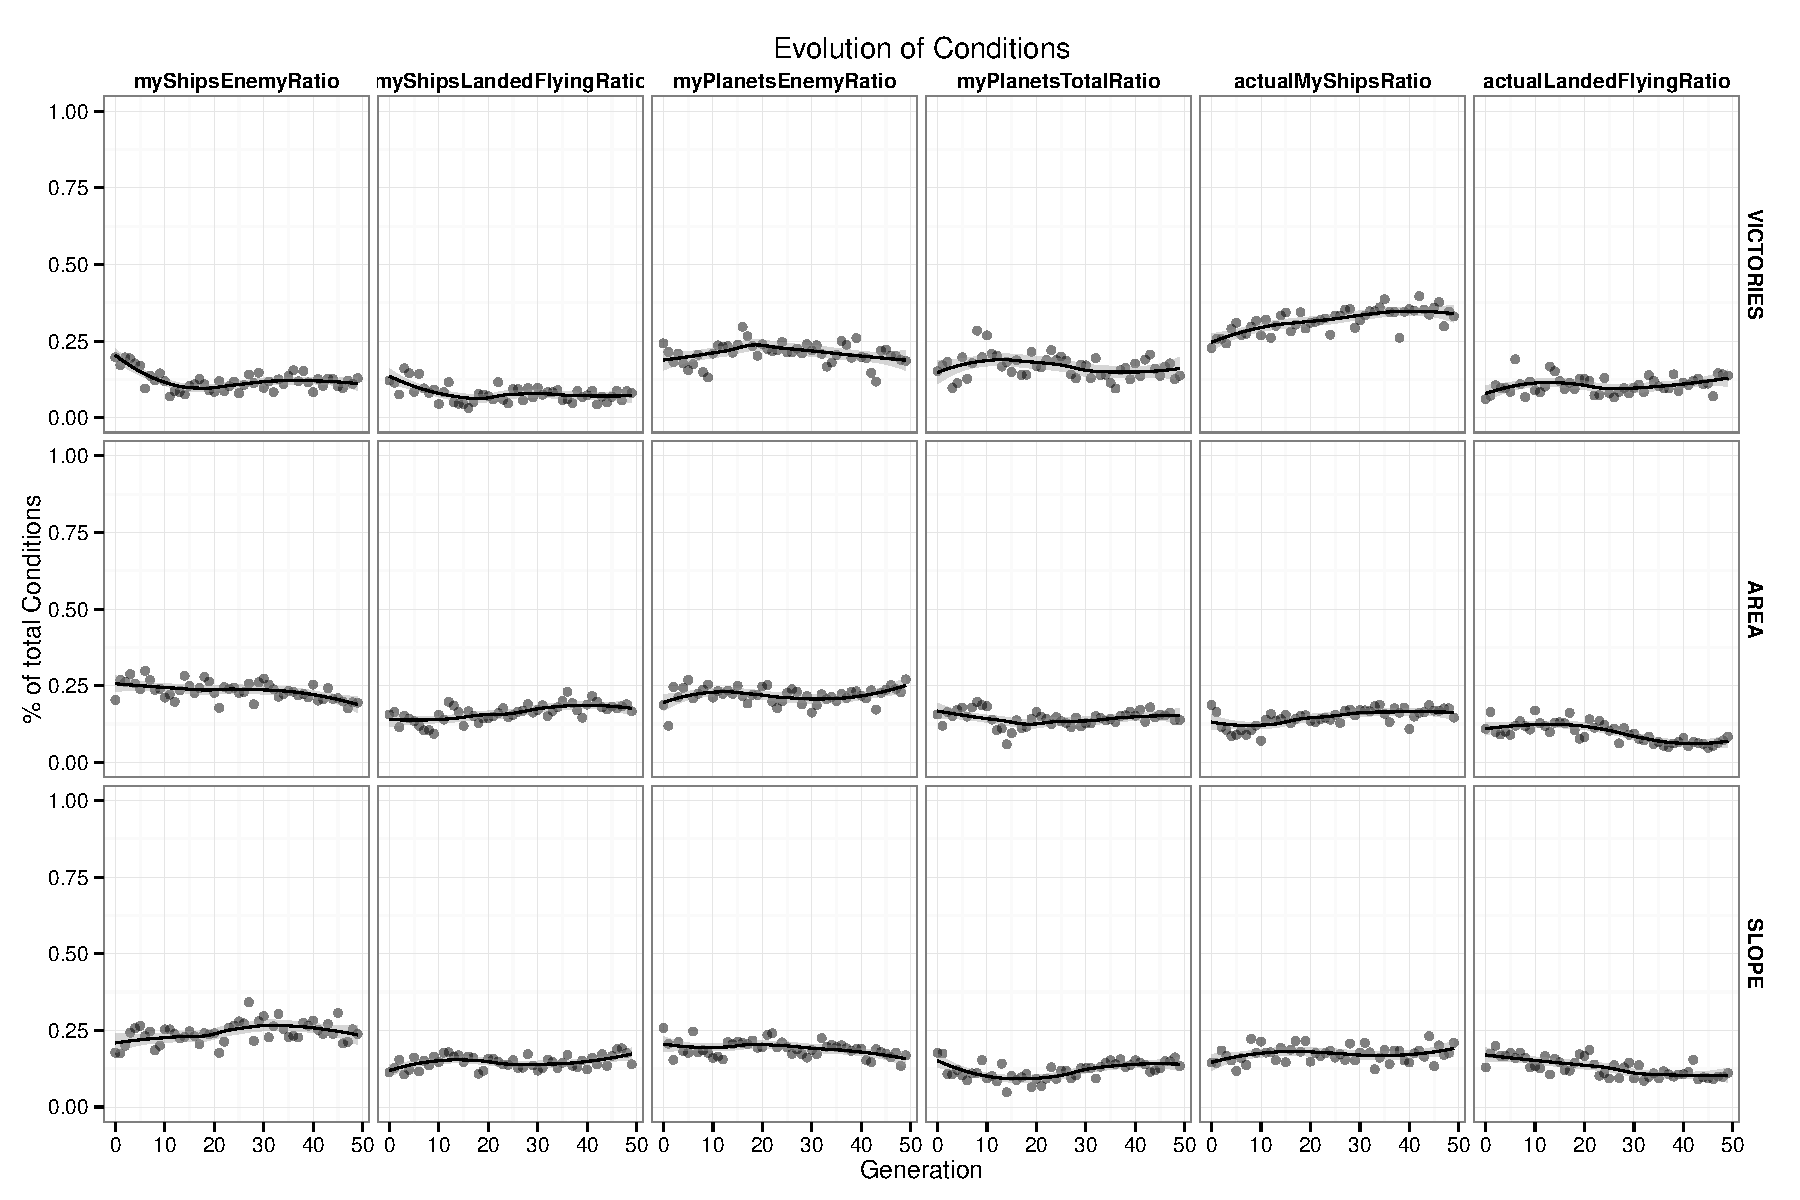
\includegraphics[width=15cm]{nuevas_imgs/estudio_CONDITIONS_s.pdf}
    }
  \end{center}
  \caption{Evolution of the percentage of every condition over the
    total of conditions used by the best individual by generation of
    every execution.} 
  \label{figura:e_conditions}
  \end{figure}

After analyzing the condition or decision type, let us examine next
{\em action type} that an agent can choose. Figure 
\ref{figura:e_actions} shows the percentage of the three types of
actions that can be performed by the agent: {\em attack}, {\em
  reinforce} and {\em doNothing}. Results clearly show that the {\em
  attack} action is the most used in all fitness methods, but it is
interesting to mention that the Victory fitness uses less times than
the others the {\em reinforcement} one with respect to attacking. 
 This
also can be explained because the number of ships is not measured
during the evaluation, unlike the other two methods, where a high
amount of ships during all the run yields a higher fitness value. 

  \begin{figure}[ht]
  \begin{center}
  \makebox[\linewidth][c]{
    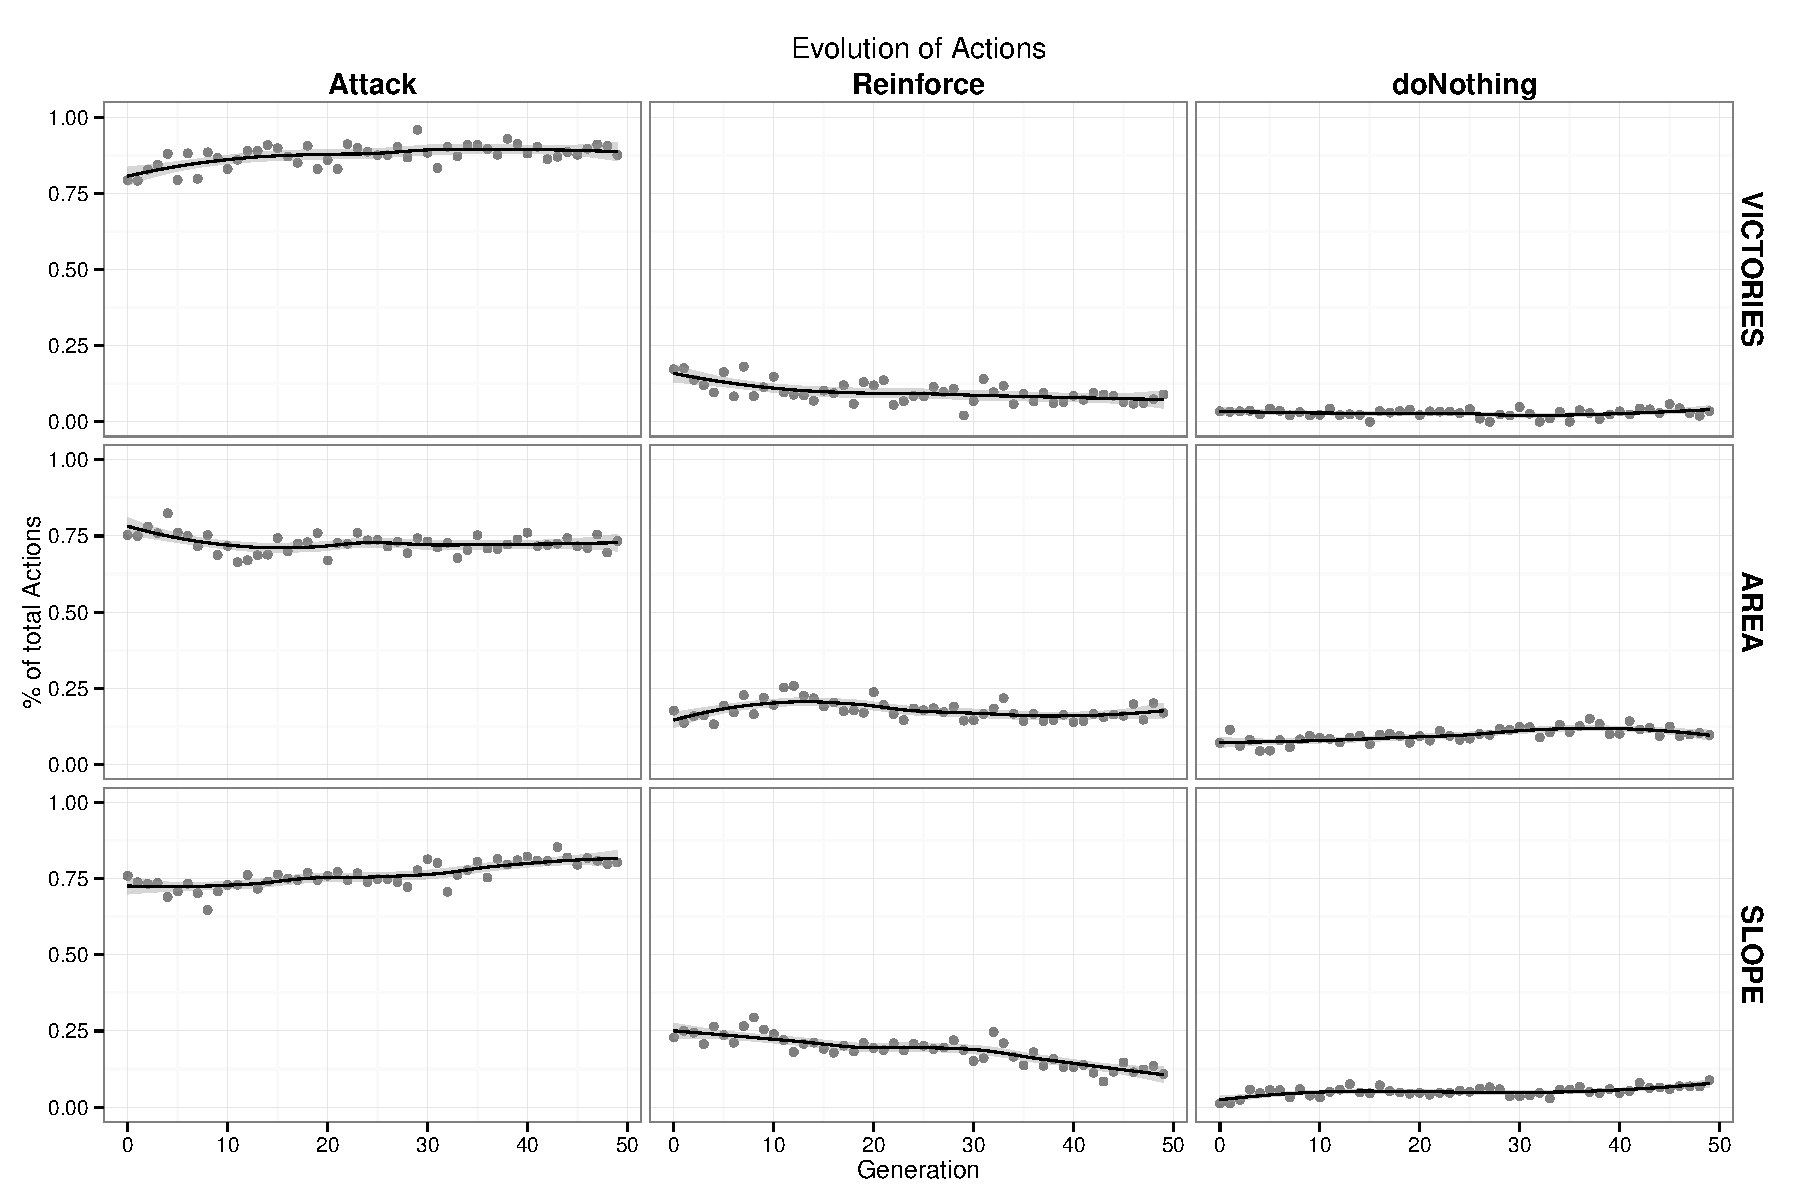
\includegraphics[width=15cm]{nuevas_imgs/estudio_ACTIONS_s.pdf}
    }
  \end{center}
  \caption{Evolution of the percentage of every type of actions over the total of actions used by the best individual by generation of every execution.
  }
  \label{figura:e_actions}
  \end{figure}

Focusing in the {\em type of attacks}, Figure \ref{figura:e_attacks} shows that the \emph{attack\_Nearest} action is the most used one in the Victory fitness, because this action is very beneficial in order to get a fast win, as this fitness function promotes. The reason is that, normally, it takes less time to conquer a close planet than a farther one. The interesting fact is that this type of attack seems to be a better option than the similar \emph{attack\_Weakest} (low number of ships to be conquered) or \emph{attack\_Quickest} (easy to be conquered).

On the contrary, in Slope and Area fitness, attacking the enemy planets with the 
highest growing ratio ({\em wealthiest}) and the ones with high growing ratio but low number of ships ({\em beneficial}) imply less ships for the enemy and more for the player in the following turns, and therefore, a higher fitness value, so they are selected more frequently. 
As it could be expected, {\em attacking random planets} do not seem to be a good strategy in any of the methods compared. Attacking the base is not a good strategy neither, even if it was considered as one of the most important actions in previous works that do not use Genetic Programming \cite{Mora_noisy_jcst}.

  \begin{figure}[ht]
  \begin{center}
  \makebox[\linewidth][c]{
    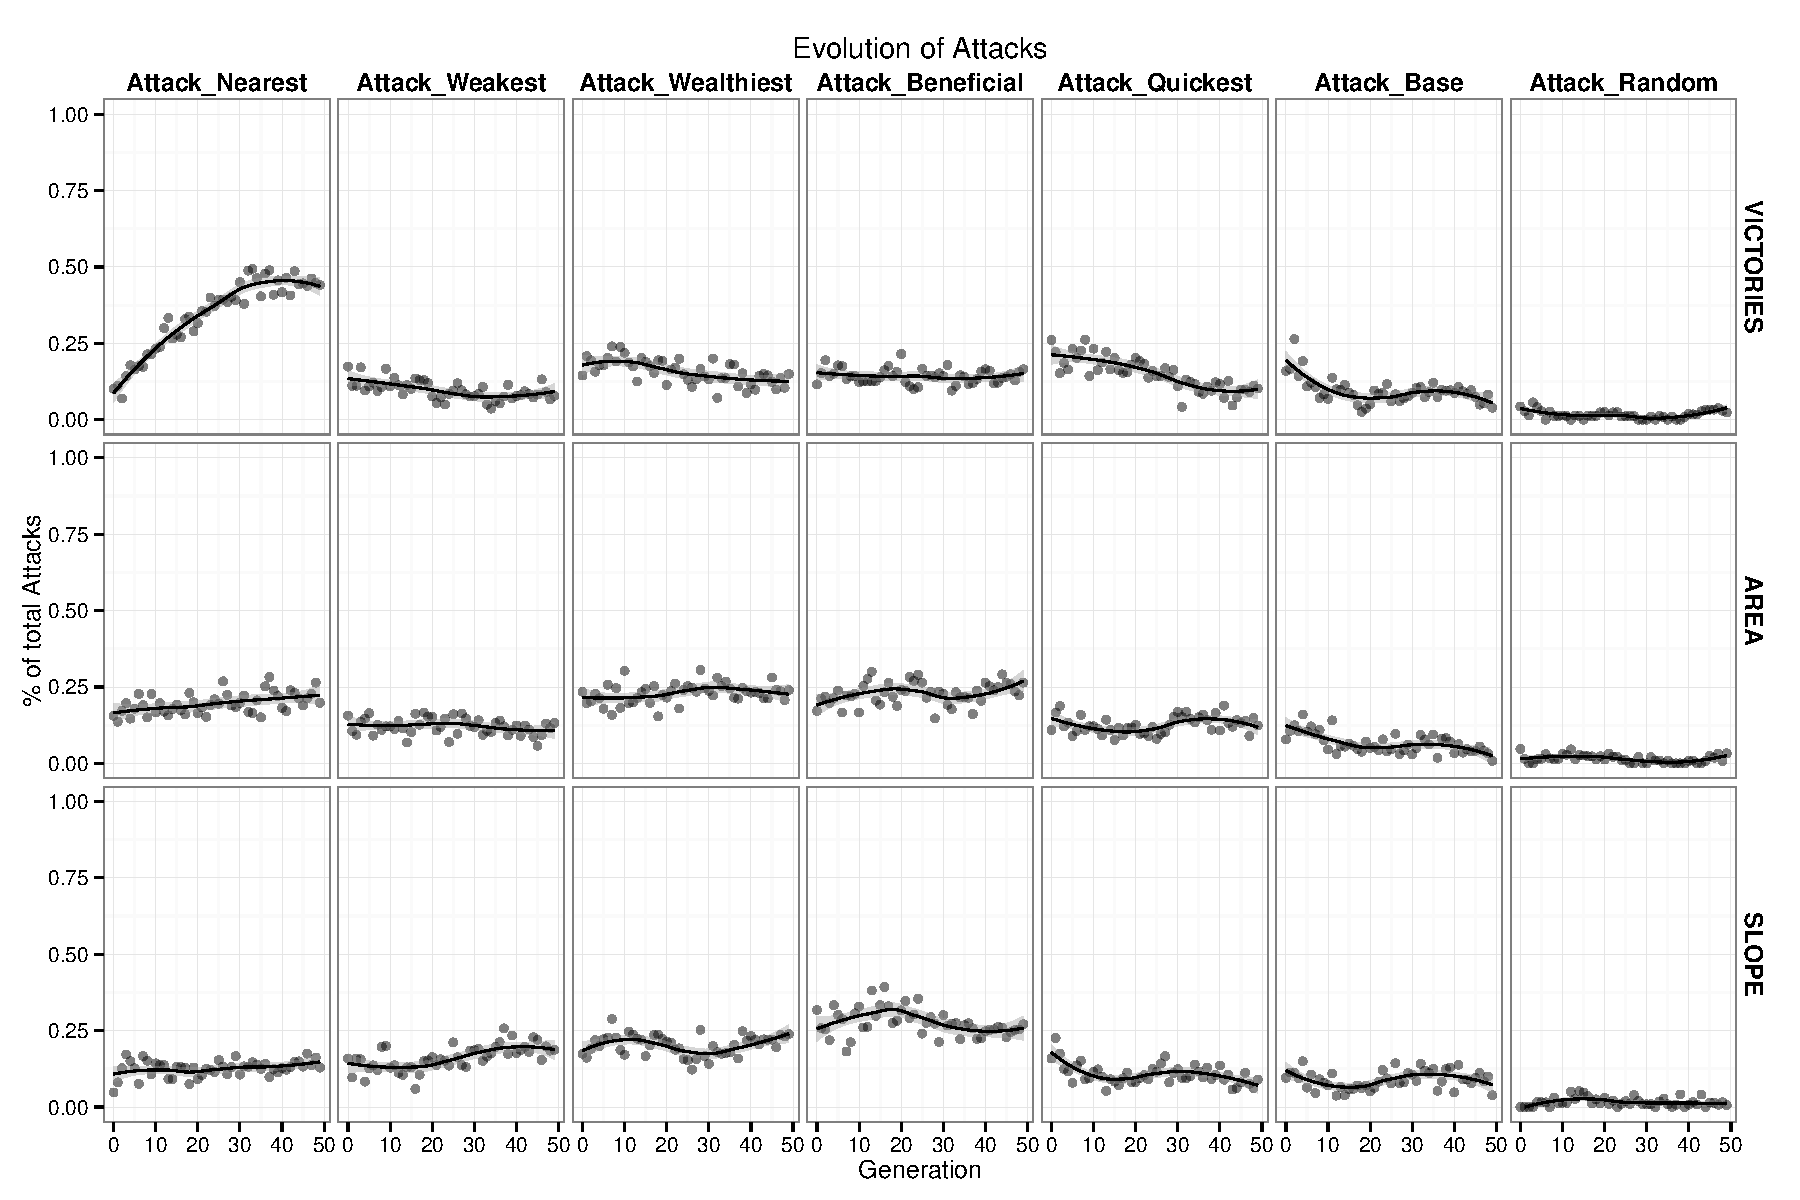
\includegraphics[width=15cm]{nuevas_imgs/estudio_ATTACKS_s.pdf}
    }
  \end{center}
  \caption{Evolution of the percentage of every type of attack over the total of attacks used by the best individual by generation of every execution.
  }
  \label{figura:e_attacks}
  \end{figure}

With respect to the {\em target chosen} in every attack, Victory fitness is again focused on destroy the enemy as quickly as possible (\emph{Target\_EnemyPlanet}), avoiding the neutral ones, while the other two methods (Area and Slope) seek any kind of planet to increase their number of ships during the match.

   \begin{figure}[ht]
  \begin{center}
  \makebox[\linewidth][c]{
    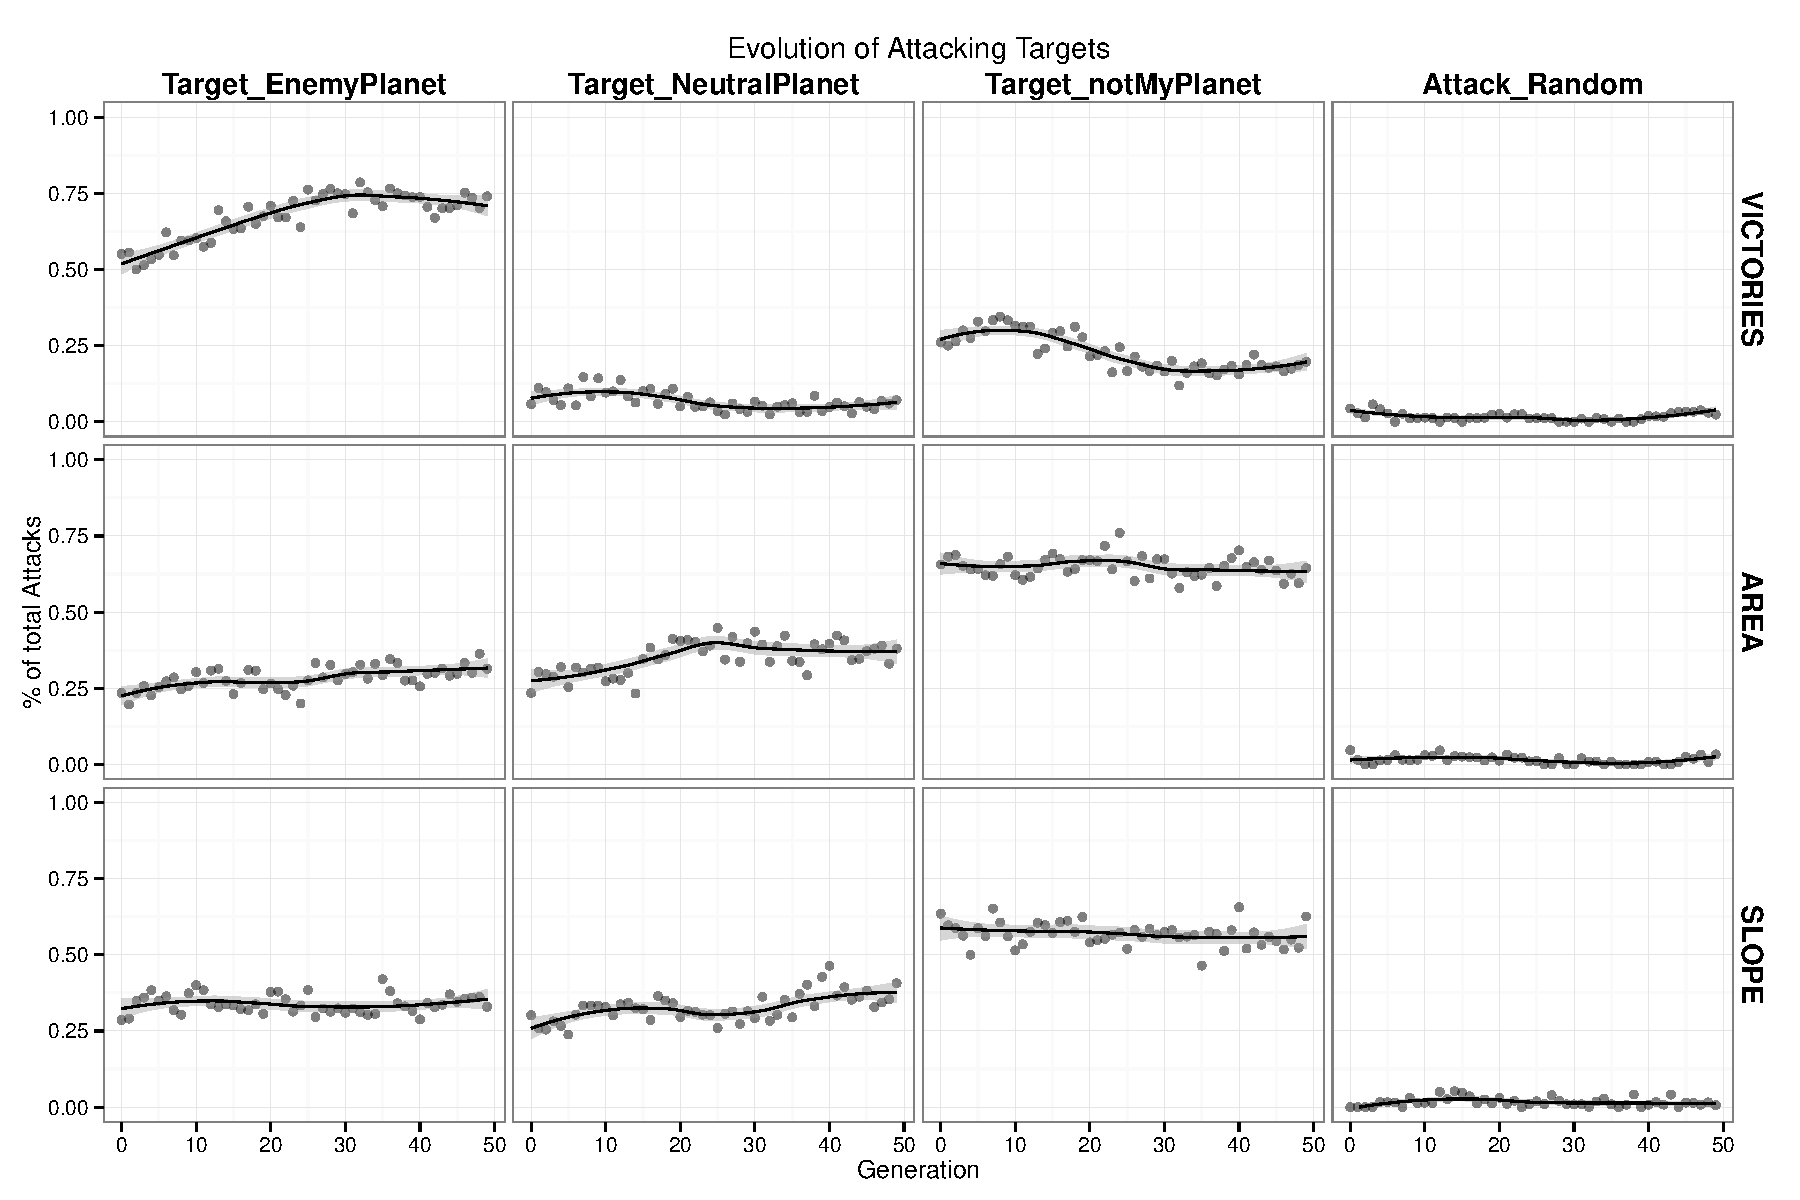
\includegraphics[width=15cm]{nuevas_imgs/estudio_TARGETS_s.pdf}
    }
  \end{center}
  \caption{Evolution of the percentage of every type of attacking targets over the total of attacks used by the best individual by generation of every execution.
  }
  \label{figura:e_targets}
  \end{figure}


Finally, and concerning the {\em reinforce} action, the three methods create bots that prefer to reinforce nearest planet (\emph{Reinforce\_Nearest}), as shown in Figure \ref{figura:e_targetsReinforce}. This is useful, as travelling ships cannot be used for attack or defence, and minimise this time can be more efficient if used to attack instead reinforce distant planets. However, during the evolution of the Victory fitness a higher oscillation of these percentages can be seen. As previously explained, the bots generated with this method are not focused on the reinforce action, so this number is not maintained during the run. 
It can be seen that \emph{Reinforce\_Base} gets less relevant for the best individuals, since this is less useful if the bot tries to expand its owned planets.

    \begin{figure}[ht]
  \begin{center}
  \makebox[\linewidth][c]{
    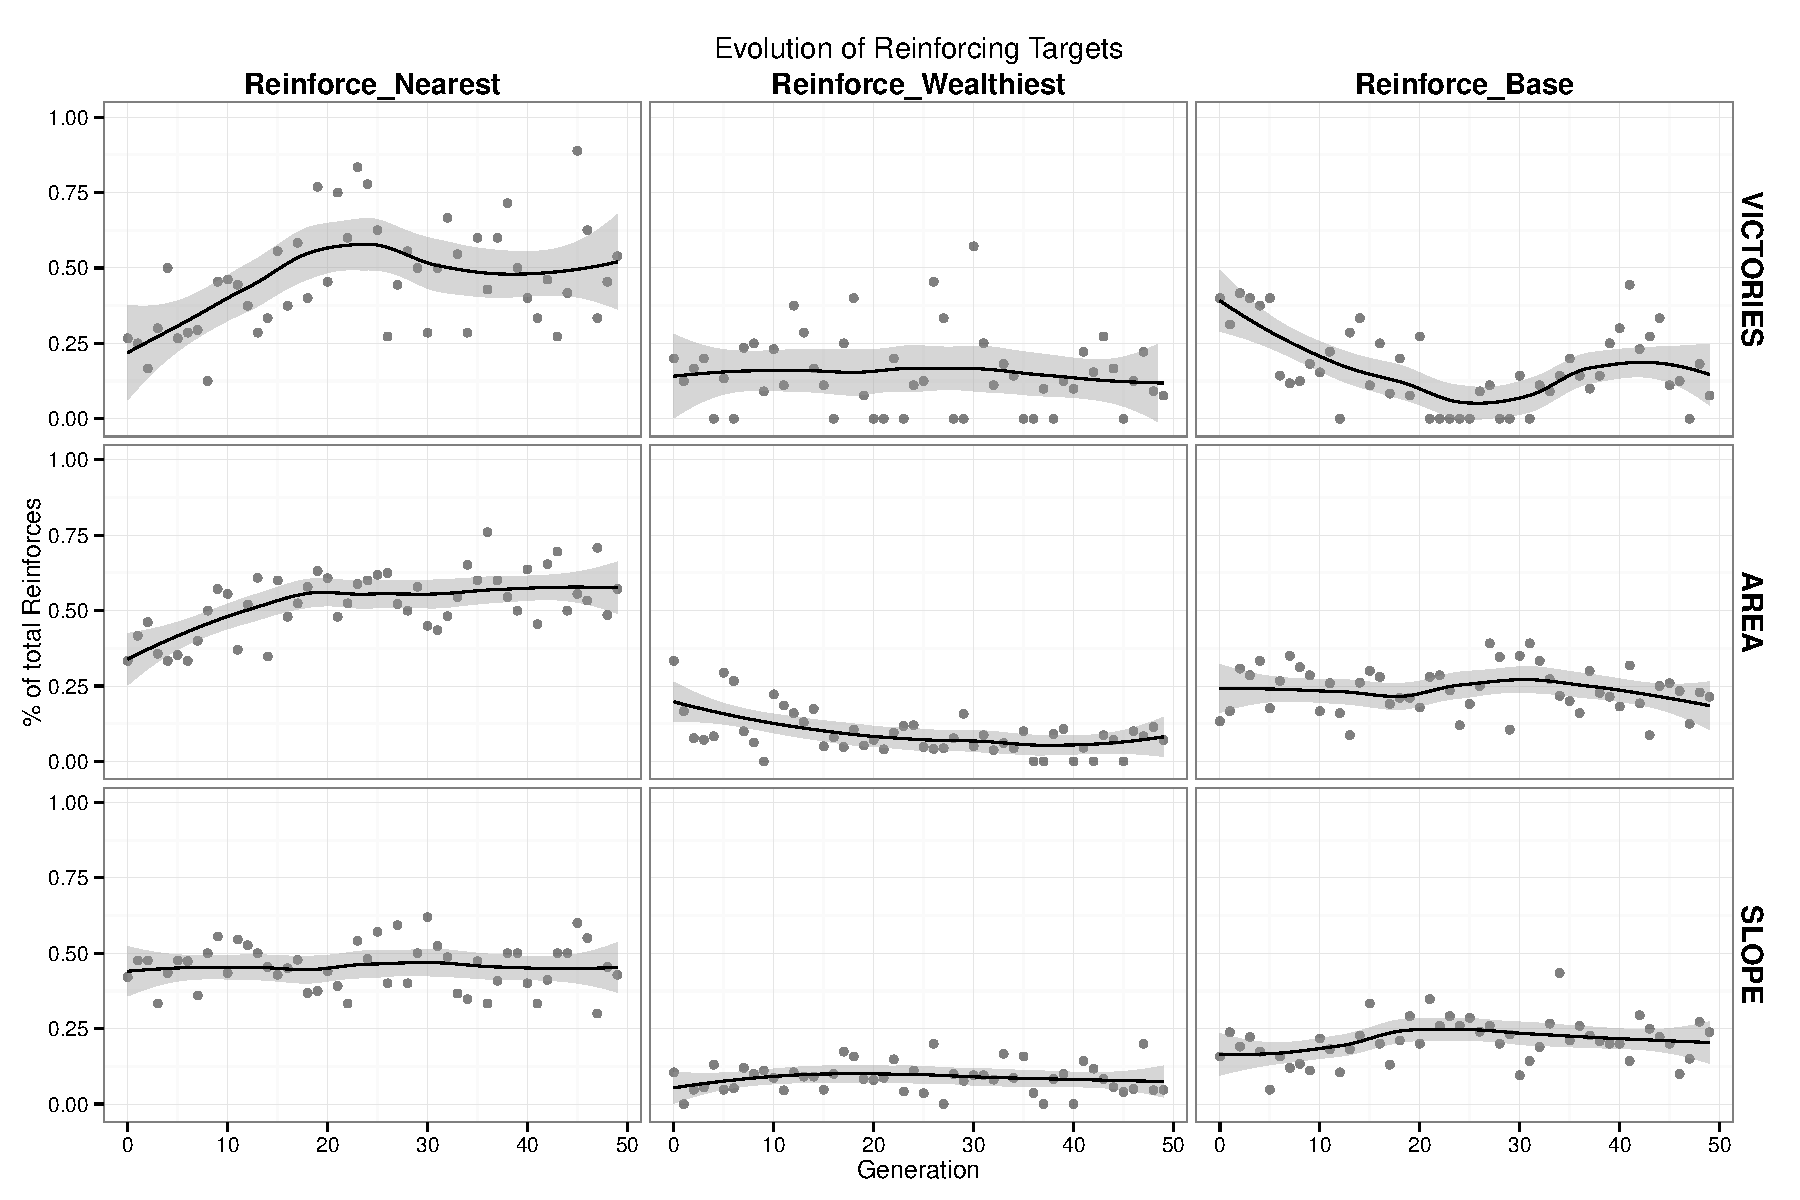
\includegraphics[width=15cm]{nuevas_imgs/estudio_TARGETS_REINFORCE_s.pdf}
    }
  \end{center}
  \caption{Evolution of the percentage of every type of reinforcement over
    the total of reinforcements used by the best individual by generation
    of every execution}
  \label{figura:e_targetsReinforce}
  \end{figure}

This study could be useful for an expert (player) which can analyse the most used actions by the best individuals and extract new knowledge from them. For instance, according to these results, most desirable actions are those which minimise the time that the ships are flying (not in a planet).
Moreover, the fact that none rule has disappeared in the evolutionary process would mean that they are correct, and thus, that the expert knowledge is accurate and useful.


%-----------------------------------------------------------------
%%%%%%%%%%%%%%%%%%%%%%%% CONCLUSIONS %%%%%%%%%%%%%%%%%%%%%%%%%%%%%
%----------------------------------------------------------------- 
\section{Conclusions}
\label{sec:conclusion}

The objective of this work is to validate which is the best approach to evaluate individuals in a Genetic Programming algorithm designed to create competitive bots for a RTS game named Planet Wars. To this aim, three different fitness functions have been studied and compared in different ways: analysing the evolution of the individuals (bots) along the generations, their tolerance to noise/uncertainty, the changes and improvements in their behavioural models (Decision Trees, DTs), and also testing their performance against other external rivals. The functions are based on victories or in other factors present in the battles, so they are Victory-based, Slope-based and Area-based. 
 
In order to evaluate the quality of the generated agents, a competitive bot
available in the literature (GENEBOT) has been considered to fight against it. This bot was the best one obtained in an evolutionary process which optimised different parameters inside a human-designed behavioural engine.  

With respect to the evolutionary process, all the functions seem to work properly, as there is an average improvement in the population along generations, even in the presence of noise. The Victory-based fitness behaves more robustly than the other methods, while the Area-based fitness seems to be less sensitive to noise, and achieves a better percentage of victories in more generated bots than the other functions.

The analysis of the obtained rules (DTs) also shows interesting differences in the generated individuals depending on the fitness considered: 
On the one hand, the Victory-based fitness creates more balanced trees in terms of number of nodes and depth, but the actions of the best individuals obtained are more focused in a quick win, performing a more aggressive and fast play. 

On the other hand, as Slope-based and Area-based are methods that take into account the number of ships during the run, they promote to attack the planets with a higher growth rate (being enemies' or not) and reinforce their own planet more frequently than the Victory-based fitness. 

Although the latter function generates bots able to win more times against the bot used for training (GENEBOT), when confronting all the generated bots between them, those generated by the Area-based fitness win more times. The reason is that there exists a higher variation in depth and number of nodes in the Victory-based produced bots, 

implying more behavioural differences, and probably, that keeping a
high number of ships during all the match implies the bot can resist
better to the fast and aggressive attacks that Victory-based bots
tends to do. 

As future lines of work, other rules will be added to the proposed algorithm. For example, some of them analysing the map or taking into account distances between planets. More competitive enemies will be used for the evaluation in order to also yield more competitive bots. 
In addition, the approaches could be implemented and tested in more complex RTS games, such as StarCraft, or even in different videogames like Unreal\texttrademark~ or Super Mario\texttrademark~. We will also use other ways of dealing with the uncertainty/noises in the evaluation, such as using a Wilcoxon-based method to compare the individuals \cite{merelo2016statistical}. 

The analysis of DTs could be also extended to study `internal relationships' between conditions and actions, such as if a specific action (or set of actions) is always preceded by one or more specific conditions. This could yield interesting conclusions for the experts.



%%%%%%%%%%%%%%%%%%%%%%%%%%%%%  ACKNOWLEDGEMENTS %%%%%%%%%%%%%%%%%%%%%%%%%%%%%%%%
\section*{Acknowledgements}
This work has been partially funded by projects EPHEMECH (TIN2014-56494-C4-3-P, Spanish Ministry of Economy and Competitiveness), KNOWAVES (TEC2015-68752, Spanish Ministry of Economy and Competitiveness and FEDER), PROY-PP2015-06 (Plan Propio 2015 UGR), and MOSOS (PRY142/14, Fundaci\'on P\'ublica Andaluza Centro de Estudios Andaluces en la IX Convocatoria de Proyectos de Investigaci\'on).

\bibliographystyle{elsarticle-num}
\bibliography{gpbot-fitness-entcom}
\end{document}
